\documentclass[a4paper,
	11pt,
	twoside,	 % alternativ twoside, falls doppelseitiger Ausdruck erwünscht ist
    openright,
	cleardoublepage=plain,
    surpressfirstparskip,
	parskip=half,
	headings=normal,
	numbers=noenddot,
	listof=totoc,
	bibliography=totoc,
	appendixprefix,
	headsepline,
	footsepline=false,
	titlepage
	]{scrbook}

% Bitte beachten: In den folgenden Umgebungen müssen Umlaute in der Form
% {\"A}, {\"a}, {\"o} usw. eingegeben werden.
\renewcommand{\title}{Approximative Linear t-SNE Using k-Means}
\renewcommand{\author}{}
\newcommand{\email}{}

\usepackage{scrpage2}
\usepackage[table]{xcolor}
\usepackage[utf8]{inputenc} % Eingabekodierungen
\usepackage[T1]{fontenc}
\usepackage[ngerman,english]{babel}
\usepackage{url}
\usepackage{setspace}
\usepackage[export]{adjustbox}% http://ctan.org/pkg/adjustbox
%\usepackage{graphicx}
\usepackage{bibgerm}
\usepackage{booktabs}
\usepackage{microtype}
\usepackage{lmodern}
\usepackage{amssymb}
\usepackage{float}
\usepackage{mathtools}
% \usepackage{algorithmicx}
\usepackage{algorithm}
\usepackage{algpseudocode}
\usepackage[bottom]{footmisc}
\usepackage{pdfpages}
\usepackage{subcaption}
\usepackage{ltxtable}
\usepackage{listings}
\usepackage[scaled=.8]{beramono}
\usepackage{lscape}
\usepackage{longtable}
\usepackage{xhfill}
\usepackage[group-separator={,}]{siunitx}

\usepackage{blindtext}

\typearea{12}

\usepackage{xr-hyper}
\usepackage[
	breaklinks=true,
	citecolor=black,
	linkcolor=black,
	urlcolor=black,
	extension=pdf,
	english]{hyperref}
\hypersetup{
	pdfview=FitV,
	pdfstartview=FitV,
	bookmarksnumbered=true,
	pdfauthor={\author},
	pdftitle={\title}
}
\externaldocument[A-]{appendix}

\usepackage{cleveref}

% Fußnoten durchgehend numerieren
\usepackage{remreset}
\makeatletter
\@removefromreset{footnote}{chapter}
\makeatother

\deffootnote[1em]{1em}{1em}{\textsuperscript{\thefootnotemark}\,}

\tolerance=5000

\clubpenalty10000
\widowpenalty10000
\displaywidowpenalty=10000


\makeatletter
\@addtoreset{algorithm}{section}% algorithm counter resets every section
\makeatother
\renewcommand{\thealgorithm}{\thesection.\arabic{algorithm}}% Algorithm # is <chapter>.<algorithm>

\newcommand*{\fullref}[1]{\hyperref[{#1}]{\cref*{#1},~\nameref*{#1}}}
\newcommand*{\Fullref}[1]{\hyperref[{#1}]{\Cref*{#1},~\nameref*{#1}}}

\renewcommand*\Call[2]{\textproc{#1}(#2)} % fix for nested calls
\newcommand{\detto}[1][.4pt]{\xrfill{#1}~\textquotedbl~\xrfill{#1}}

\begin{document}
\pagenumbering{Roman}

% Titelseite.
\includepdf{../titelblatt.pdf}
\thispagestyle{empty} % no II on backside of title page

\frontmatter

\onehalfspacing
\setcounter{tocdepth}{2}

\chapter*{Abstract}

Dimensionality reduction is the transformation of high-dimensional
data into a lower dimensional space while keeping the interesting parts
of the data intact. Ideally, the low-dimensional so-called embedding
reveals structure that would have been much more difficult to detect
in the high-dimensional space.

There are many different approaches to dimensionality reduction, and the most
common taxonomy separates them into linear and non-linear methods. Linear
methods transform the high-dimensional data solely by applying linear
transformations, such as PCA, while non-linear methods are essentially
free to transform the data by any means.

In this thesis, we will be focusing on a non-linear method called $t$-SNE,
which is a variant of Stochastic Neighborhood Embedding using the Student-$t$
distribution. $t$-SNE has become popular due to the visual properties of the
embeddings it produces: well-separated clusters consisting of similar items.
It is, however, a stochastic method, non-parametric in its original form, possesses
a difficult to optimize non-convex objective function and also has a prohibitively
high runtime complexity of $\mathcal{O}(n^2)$.

We implement and evaluate a variant of $t$-SNE named $kt$-SNE utilizing $k$-Means
and locality sensitive hashing. We achieve an overall runtime complexity of $\mathcal{O}(n)$.
We thoroughly evaluate our method and put it to the test against three competing
methods. Our method achieves results that are mostly within 10\% of the best result of the
competing methods on real data and runs significantly faster than Barnes-Hut $t$-SNE.


\vfill
\pagebreak
\thispagestyle{empty} % no II on backside of title page

\chapter*{Zusammenfassung}

Unter Dimensionsreduktion versteht man die Transformation von hochdimensionalen
Daten in einen niedrigdimensionalen Raum, ohne die wesentlichen Merkmale der Daten
zu verlieren. Idealerweise gibt das niedrigdimensionale sogenannte Embedding seine
Struktur leichter Preis als sein hochdimensionales Gegenstück.

Es gibt viele unterschiedliche Ansätze zur Dimensionsreduktion. Die häufigste Unterscheidungsmethode
ist zwischen linearer Dimensionsreduktion und nonlinearer Dimensionsreduktion. Lineare
Dimensionsreduktionsmethoden transformieren die Daten in einen niedrigdimensionalen Raum
nur unter Verwendung von linearen Transformationen, wohingehen nonlineare Methoden die
Daten jegliche Art von Transformation anwenden dürfen.

In dieser Thesis beschäftigen wir uns mit einer nonlinearen Methode namens $t$-SNE, die
eine Variante von Stochastic Neighbor Embedding (SNE) unter Verwendung der Student-t Verteilung
darstellt. $t$-SNE ist beliebt aufgrund der visuell ansprechenden Embeddings, die Clusterings
ähneln, die es produziert. Allerdings ist sie auch stochastisch, nonparametrisch, verfügt
über eine schwierig zu optimierende Zielfunktion und hat zudem noch eine hohe Laufzeitkomplexität
von $\mathcal{O}(n^2)$.

Wir implementieren und evaluieren einer variante von $t$-SNE namens $kt$-SNE,
die den Clusteringalgorithmus $k$-Means und Locality Sensitive Hashing
verwendet. Wir erreichen eine Laufzeitkomplexität von $\mathcal{O}(n)$. Wir
evaluieren unsere Methode gründlich und vergleichen sie mit drei vergleichbaren
Methoden. Unsere Methode erreicht Resultate die zumeist innerhalb von 10\% der
besten Methode auf realen Daten liegen und läuft signifikant schneller als
Barnes-Hut $t$-SNE.


\vfill
\pagebreak
\thispagestyle{empty} % no II on backside of title page

% Inhaltsverzeichnis
\tableofcontents

\mainmatter

% Hauptteil der Arbeit
\chapter{Introduction}\label{ch:intro}

Dimensionality reduction is an important tool of data analysis. High dimensional
data sets may encompass so many dimensions that it becomes difficult to understand
let alone interpret the data. Dimensionality reduction can help by reducing the dimensions
such that the data can be drawn or can be used as a means of feature extraction so that
other methods, e.g. classification algorithms, get better footing and produce better
results.

Dimensionality reduction has been studied for more than a hundred years with PCA~\cite{pearson_pca}
being the most prominent and also one of the oldest methods. PCA belongs to the
class of \emph{linear} dimensionality reduction methods, sometimes also referred
to as \emph{projective} dimensionality reduction. Linear dimensionality reduction (LDR)
finds a projection $P$ to transform the data into a lower dimensional space. This
method is only effective if whatever property should be preserved can be represented
linearly.

Nonlinear dimensionality reduction (NLDR) is used when this is not the case. There
exist multiple approaches to NLDR, e.g. kernel PCA which is a projective method but
in a feature space possibly resulting from a nonlinear mapping, but the method we will
be focusing on is \emph{manifold learning}. The idea of manifold learning is that
the high dimensional data sets is artificial and most of the data actually lies on
a much lower dimensional manifold plus some noise. Most manifold learning methods
do not actually learn the manifold itself but try to approximate the geodesic distance
across the manifold, often by computing a $k$-nearest neighbor graph. As such, a surprising
amount of manifold learning methods are actually more or less graph embedding algorithms after
the initial step of computing the graph which differs between methods. Of course, many graph
embedding methods are not designed to produce ``good-looking'' low dimensional embeddings
and are instead used as means of feature extraction, and deal with different features and problems inherent
to graphs.

A particularly prominent nonlinear dimensionality reduction method is
$t$-SNE~\cite{tsne}.  $t$-SNE has found widespread usage in many scientific
communities dealing with high-dimensional data, such as gene-expression data.
$t$-SNE has the property that similar points appear to be clustered in its
output, which is visually pleasing and thus readily accepted as a good
embedding, even if limitations apply~\cite{art_tsne,misread_tsne}. As such, it
is also considered to be a visualization technique. However popular, $t$-SNE
comes with a significant downside: its high computational complexity---of
quadratic order---make it unusable for particularly large data sets.

\section{Motivation}

The high computational cost of $t$-SNE is the main motivation of this thesis.
There have been multiple attempts at speeding it up~\cite{bhtsne,fitsne,umap,largevis}
and in this thesis, we introduce another way of doing so and compare ourselves
against the other methods.

$t$-SNE can be divided into two phases. The initial phase consists of computing
probabilities in the high dimensional pairs. This involves finding all, or at
least \emph{some}, distances to all other points or a selected few nearest
neighbors. The approach to optimize this is to use only \emph{approximate}
nearest neighbors. This can be done by e.g. using trees, as done in Barnes-Hut
$t$-SNE~\cite{bhtsne}, or in FIt-SNE~\cite{fitsne}, or by any other approximate
nearest neighbor finding scheme. We choose to use locality sensitive hashing, a
well established method used in many fields such as duplicate detection (e.g.
plagiarism detection), clustering, audio similarity detection, and nearest
neighbor search.

The second phase consists of gradient descent. In every iteration, an $n$-body
simulation is computed---the standard variant of $t$-SNE considers all forces
between all points in the data set. A simple method of speeding this up is to
coarsen the data set such that only interactions between much fewer than $n$
entities need to be computed. In Barnes-Hut $t$-SNE, this is again done with
the help of trees---each node in the tree that fulfills a quality requirement
(specified by the user) is summarized. We propose a simpler method of running
only few iterations of a clustering algorithm to find a rough segmentation of
points, where every segment can be summarized. This method of approximation can
be expected to be less precise, but also faster.

Our claim is that this rough segmentation is enough to produce an embedding in
which enough of the characteristics of the data set are represented to make
deductions, which is useful for experimental data analysis.

\section{Contribution}

We propose an accelerated approximative variant of $t$-SNE. The
algorithm utilizes locality sensitive hashing and $k$-Means to achieve
an overall linear runtime.

Our algorithm achieves embeddings that are within 10\% of the nearest
neighborhood purity achieved by the other methods. We are faster than
Barnes-Hut $t$-SNE, but fall significantly behind FIt-SNE and are roughly
as fast as UMAP. The results of our algorithm tend to be distorted, but
the underlying structure found by the other methods is also present.

\section{Structure of Thesis}

In Chapter~\ref{ch:prelim} we review the basic definitions and notations
used in this thesis, as well as introduce locality sensitive hashing, $k$-Means
and stochastic neighborhood embedding (SNE). Our work builds upon these methods
and thus an basic unterstanding is required.

In Chapter~\ref{ch:related-work} we survey various important methods of
dimensionality reduction. We review both linear and nonlinear methods, with a
focus on the latter.  Next, we discuss our proposed algorithm and explain it in
relation to $t$-SNE, on which it is based, in Chapter~\ref{ch:main}. Our
method is evaluated in Chapter~\ref{ch:eval}. We tune the parameters of our
method and compare it against other selected methods on real and synthetic data
sets. We discuss our findings and conclude this thesis in chapter~\ref{ch:end}.

\chapter{Preliminaries}\label{ch:prelim}

\section{Definitions and Notation}

Dimensionality reduction maps high-dimensional data points $\{ x_i \}_{i=1}^{n}
\in \mathbb{R}^d$ to low-dimensional points $\{ y_i \}_{i=1}^{n} \in
\mathbb{R}^r$ where $r \ll d$ such that the points $Y$ ``represent'' the points
$X$. The low-dimensional representation is called the embedding. How faithfully
the embedding represents the core properties of the data is the property to
optimize.  What constitutes a faithful embedding is the fundamental question of
dimensionality reduction and there are multiple answers.

Linear dimensionality reduction methods often deal with the variance. The supposition is
that variance constitutes important structure and thus, a faithful embedding should preserve the
variance. Other methods assume that the data actually lies on a lower dimensional manifold which
is locally linear but possibly globally nonlinear. The intrinsic dimensionality of the manifold
is the dimensionality of the space into which the data should be embedded. Note that the structure
of the manifold and its dimensionality is fundamentally unknown and must be supplied as an
input parameter---i.e. the problem of dimensionality reduction is ill-posed.

For linear dimensionality reduction we write the matrices as $X^{d \times n}$, i.e. the
observations are in the columns. This makes some notation easier and is common practice
in this field, although it may confuse computer scientists that are more used to having
the observations as rows. For almost all methods a centering is required, so we simply
assume that $X$ is already centered, i.e. its mean is zero.

A common element in the problem definitions is the covariance matrix $XX^T \in \mathbb{R}^{d \times d}$ which is
often manipulated (e.g. decomposed) to maximize the overall variance or minimize
the covariance of the embedding. The variances of each feature is written in the main diagonal,
while other fields contain the covariances. The trace of a matrix $\text{tr}(\cdot)$
is the sum of the main diagonal and is also the sum of the eigenvalues. This already
implies the connection between maximizing variance and choosing the largest
eigenvalues---as is done in PCA.

We always assume that the distance at hand is the Euclidean distance, $d(p,q) =
|| p - q ||_2 = \sqrt{\sum_{i=1}^n (p_i - q_i)^2}$.  Most methods use the
squared Euclidean distance.

The Frobenius norm of a matrix is written as $|| \cdot ||_F$ and is defined as
$|| A ||_F = \sqrt{\sum_i \sum_j  a_{ij}^2}$ for $A \in \mathbb{R}^{m \times n}$.

The eigendecomposition of a orthonormal matrix $A$ results into two matrices $Q$ and $\Lambda$
such that $A = Q\Lambda Q^T$. This is only applicable for diagonalizable matrices.
The generalization to all matrices is the singular value decomposition $A = U \Sigma V^T$.

A positive semidefinite matrix $M \in \mathbb{R}^{n \times n}$ is positive semidefinite
if the scalar $z^TMz$ is positive or zero for all non-zero $z \in \mathbb{R}^n$, a constraint
implying semidefiniteness is written as $M \succeq 0$.

\section{Locality-Sensitive Hashing}

Locality-sensitive hashing (LSH) is a family of hashing methods designed
to find similar items by hashing them to the same address. In a way, these
hashing methods differ from all other common uses of hashing, which try
to avoid colliding hash indices at all cost.

The need for LSH arises simply from the quadratic growth of the na\"ive
algorithm for finding similar pairs, which involves examining all possible
$\mathcal{O}(n^2)$ pairs. If an approximative solution is acceptable, this can
be sped up significantly by partitioning the space into segments by hashing the
items. These segments are then the hash buckets, and the hash function
transform the vectors into some subspace from which the bucket membership can
be derived. The contents of a bucket can be assumed to be sufficiently similar
to each other with some probability larger than $p_1$, while sufficiently
dissimilar items hash to different buckets is smaller than $p_2$. Formalizing
this, we get the definition of a locality-sensitive family of hash function
$\mathbf{F}$ and its four defining parameters $d_1$, $d_2$, $p_1$ and $p_2$:

\begin{enumerate}
  \item If $d(x, y) \leq d_1$, then the probability of collision is at least $p_1$.
  \item If $d(x, y) \geq d_2$, then the probability of collision is at most $p_2$.
\end{enumerate}

Such a family of locality-sensitive hash functions $\mathbf{F}$ is then called
$(d_1, d_2, p_1, p_2)$-sensitive~\cite{mmds}.  Intuitively, this simply
formalizes the notion that the collision probability for similar points is
higher than for dissimilar points.

Various locality-sensitive families of hash
functions can be defined for distances such as the Euclidean or Cosine
distance. LSH is widely used for data consisting of documents, with
applications such a plagiarism detection, finding (approximative) nearest
neighbors or many other tasks hinging on similarity detection~\cite{mmds},
however it can be used for any kind of data for which a locality-sensitive
family of hash functions can be defined.

A simple example of a family of hash function are signed random projections
(SRP) in hyperplane LSH. Each hash function is defined by a random vector $w$
defining a hyperplane going through the origin which divides the space into two
sub spaces. The hash function is thus

\begin{equation}
  h_w(x) = \text{sign}(w^T x).
\end{equation}

\begin{figure}[tp]
  \centering
  \includegraphics[width=.6\textwidth]{img/srp}
  \caption{Space segmented into 6 buckets by 3 random hyperplanes (SRP)}
  \label{fig:srp}
\end{figure}

Figure~\ref{fig:srp} shows a concrete example. In this case, the colored
regions each correspond to a hash bucket. A total of 3 hash functions are used,
each corresponding to one of the thick dashed lines delimiting the colored regions. Multiple
hash tables, each with their own three hash functions, would be used and the
union of all hash buckets that match a query object would form the candidate
set, whose contents would be ranked by the distance to the query object. A
similar example consists of randomly projecting a point onto a line which is
segmented into buckets. More exotic variants of LSH with different means of
partitioning the vector space also exist, such as clustering
LSH~\cite{lshcomp}, but it should be noted that finding the collision
probabilities becomes significantly difficult~\cite{pstablelsh} even for the
previous example of a segmented line.

A notable family of locality sensitive hash functions which were used in our is
Cross-Polytope LSH. %TODO

An important modification to standard LSH, beside the multitude of different
families of hash functions, is multi-probe LSH~\cite{multiprobelsh}. Multi-probe
LSH reduces the overhead due to the need of many hash tables---many in this
case refers to hundreds for high-dimensional data---to increase query result
quality by probing multiple buckets where similar items could have been
misplaced. This increases the size of the candidate pool without allocating
additional hash tables and is thus a simple but effective optimization that has
been widely adopted.

\section{k-Means}

$k$-Means is a simple and popular clustering method for data with a known
amount of clusters ($k$). It works by assigning points to the nearest
cluster-mean (centroid), updating the cluster mean after all points have been
assigned, and repeating this process until a stopping criterion is met,
this could either be the convergence of the sum of squared distances to the centroids---equivalent
to the centroids no longer changing positions (significantly)---or something simpler such as as fixed amount of iterations. Algorithm~\ref{alg:kmeans}
briefly outlines the process.

\begin{algorithm}[tb]
    \begin{algorithmic}
      \Procedure{$k$-means}{$X$, $k$}
      \State $\text{centroids} \gets \text{initial centroids } c_1, c_2, \ldots c_k$

      \While{stopping criterion has not been met}
        \ForAll{points $p_i$ in $X$}
          \State $c_i \gets \text{closest centroid to } p_i$
          \State assign $p_i$ to $c_j$
        \EndFor

        \ForAll{centroids $c_i$}
          \State $c_i \gets \text{center of mass of all points assigned to } c_i$
        \EndFor
      \EndWhile
      \EndProcedure
    \end{algorithmic}
    \caption{$k$-Means}
    \label{alg:kmeans}
\end{algorithm}

$k$-Means is linear in the number of input points, however reaching convergence
may take many iterations. $k$-Means also has a strong assumption of
Gaussian-shaped clusters and is unable to find clusters of other shapes.
Finally, finding a suitable $k$ is not straightforward and is usually done by
rerunning the algorithm and finding an optimum sum of squared distances.

\section{Stochastic Neighborhood Embedding}

Stochastic Neighborhood Embedding (SNE)~\cite{sne} is a probabilistic
embedding method and the direct predecessor of $t$-SNE. SNE proceeds
by computing the high-dimensional asymmetric probabilities that
some point $i$ will pick another point $j$

\begin{equation}
  p_{ij} = \frac{\exp (-d_{ij}^2)}{\sum_{k \neq i} \exp (-d_{ik}^2)}
\end{equation}

where $d_{ij}^2$ are some kind of dissimilarity, possibly the scaled squared
Euclidean distance given by

\begin{equation}
  d_{ij}^2 = \frac{ ||x_i - x_j||^2}{2\sigma_i^2}.
\end{equation}

Here, the value $\sigma_i$ is either found by binary search such that the
entropy of the distribution $p_{i\cdot}$ is equal to $\log k$, where $k$
is the effective number of neighbors, most often called perplexity.

Another probability is defined in a similar way for the low-dimensional
points, defined by

\begin{equation}
  q_{ij} = \frac{\exp (-||y_i - y_j||^2)}{\sum_{k \neq i} \exp (-||y_i - y_j||^2)}.
\end{equation}

The optimization target is then to minimize the Kullback-Leibler divergence between
these two distributions.

Unfortunately, this method has quadratic runtime and is thus not viable for
large data sets. Other downsides have been found and summarized by the subsequent
$t$-SNE paper~\cite{tsne} and include the difficult to optimize objective and the
so-called crowding problem, of which the latter is amended by using a different
probability distribution in the low-dimensional space (namely the Student-$t$ distribution
instead of the Gaussian distribution). $t$-SNE is discussed in the Related Work
section of this thesis.

\chapter{Related Work}\label{ch:related-work}

In this chapter, we survey a few key dimensionality reduction methods,
including t-SNE, which our work modifies, and other algorithms that compete
with our proposed algorithm.  We include both linear methods and nonlinear
methods, though we pay special attention to nonlinear methods. We finish by
taking a closer look at the variant of LSH which was used in our work.

\section{Linear Methods}

Linear dimensionality reduction deals with finding a new basis into which
the input data can be transformed with minimal loss of important structural
information.  What is deemed to be ``important'' depends on the method---for
some, the new basis should be such that the variance of the projected data is
maximized, or alternatively, if information about labels is available, the
important information must be what separates the classes.

Linear dimensionality assumes that the underlying structure of the data is
rather simple, otherwise it would not be able to be represented as linear
combinations of the input data. This assumption implies that the variance of
the error (or the noise) is lower than the variance of the observed phenomenon.
Although this assumption is often correct and has the added bonus of
interpretability, on some data sets it is not sufficient to uncover all or even
any of the hidden structure. This raises the need for nonlinear dimensionality
reduction which is covered in later subsections.

Dimensionality reduction is usually framed in terms of optimization problems. An
objective is picked which quantifies either the presence of the desired structure
in the projected space (which should be maximized) or the deviation from the desired
state (e.g. in form of a reconstruction error, or some other form of loss), in which case
it should be minimized.

All methods covered have the added constraint that the resulting projection is
a basis, i.e. all basis vectors are orthogonal. This actually significantly
simplifies the optimization problem by limiting the search space along
orthogonal directions and allows using certain linear algebra solvers (most
notably, decomposition techniques). There exist methods that do not constrain
themselves to an orthogonal space. For a more extensive survey on linear
dimensionality reduction see~\cite{linearsurvey}.

\subsection{Principal Component Analysis}

Principal Component Analysis (PCA)~\cite{pearson_pca} is one of the oldest methods of linear dimensionality
reduction and remains the one with the most widespread usage. In its original formulation,
PCA minimized the squared residuals between the original data and the projected data. The
optimization problem is as follows:

\begin{eqnarray}
    \text{minimize} & || X - MM^TX ||_F^2 \\
    \text{s.t.} & M \in \mathcal{O}^{d \times r},
    \label{eq:pca_res}
\end{eqnarray}

More modern works (e.g. ~\cite{bishop}) detailing PCA favor a different version
of PCA whose objective function is $-\text{tr}(M^T - XX^T M)$. The solution is
equivalent to that of Equation~\ref{eq:pca_res} but results from a different
and more profound interpretation that PCA not only minimizes residuals, but
actually projects the data down into a lower dimensional space while preserving
as much variability in the data as possible. This is done by finding new linear
combinations of the features which are uncorrelated (i.e. orthogonal) and
maximize the variance, which boils down to an eigenproblem with the familiar
solution through diagonalization.

The decomposition of $XX^T$ into $Q \Lambda Q^T$ results in the optimization
problem in Equation~\ref{eq:pca_res} having an optimum when $M = Q_r$, where
$Q_r$ contains the $r$ eigenvectors in its columns which correspond to the $r$
largest eigenvalues stored in the diagonal of $\Lambda$. For a comprehensive
review of the linear algebra involved we recommend~\cite{pca_tut}.

Known weaknesses of PCA are that its runtime scales with the dimensionality of the
high-dimensional space, resulting in an overall computational complexity of $\mathcal{O}(d^3)$.  The objective function
in Equation~\ref{eq:pca_res} also results in the optimization focusing mainly on
preserving large distances in the lower dimensional space due to them having a
larger impact on the objective, which is a crucial flaw as the small distances
are usually much more important~\cite{vandermaaten_review}.

As PCA fundamentally deals with variance, it also succumbs to severe outliers
in the data due to the $L_2$ norm further exaggerating large distances. To deal
with this, multiple instances of robust PCA~\cite{robust_pca_pp_li_chen,robust_pca_galpin,
robust_pca_gao,r1_pca, pca_pp,robust_pca_candes,linearsurvey} have been proposed, mostly by shifting from the
$L_2$ norm---the traditional PCA---to the $L_1$ norm. However, this entails a
much higher computational need: an exact solution to $L_1$-PCA has an
exponential runtime, and approximation algorithms proposed so far seem to
struggle with finding acceptable solutions when the number of features $p$ is
high~\cite{pca_pp}.

The solution of PCA has also been made sparse by adding a LASSO penalty to the
objective, resulting in the objective $|| X - MM^T X ||_F^2 + \lambda || M ||_1$.
This cannot be solved by the eigenvalue approach detailed above, which led to
new algorithms~\cite{linearsurvey}. %% TODO CITATIONS linsurvey

% TODO probabilistic pca
Another important variation of PCA is probabilistic PCA~\cite{probabilistic_pca} (PPCA). The fundamental
idea is that PCA can be reformulated as the solution maximizing the likelihood of a probabilistic
latent variable model, which can be efficiently solved using an EM algorithm. Besides being efficient,
probabilistic PCA can also handle missing values and can also be used generatively to provide
new samples from the distribution~\cite{bishop}. Note that the manifold found by PPCA is arbitrary,
i.e. $M \in \mathbb{R}^{r \times n}$. A closed-form maximum likelihood solution also exists~\cite{probabilistic_pca},
but the EM algorithm is usually preferred especially if $d \gg r$~\cite{linearsurvey}.

\subsection{Multidimensional Scaling}

Multidimensional Scaling (MDS)~\cite{torgerson} is a an entire class of linear
dimensionality reduction methods following a slightly different idea. Instead
of minimizing the residuals of the projection, we compute pairwise similarities
(or dissimilarities) of the data and compute a mapping into a space such that
these similarities are approximated. The classical MDS (sometimes shortened to
CMDS, although this is sometimes misleading, or simply classical scaling~\cite{vandermaaten_review}) optimization program, however, is
simpler, and instead maximizes the scatter in the projected space~\cite{linearsurvey} in the belief
that such an projection is the most informative one:

\begin{align}
    \text{maximize} \quad & \sum_i \sum_j ||M^T x_i - M^T x_j||^2\\
    \text{s.t.} \quad & M \in \mathcal{O}^{d \times r} \nonumber
\end{align}

It is easy to see that this maximization of scatter and the maximization of
variance in PCA leads to the same solution~\cite{cox_mds, borg_groenen_mds}.
However, classical scaling scales with the number of points $n$ which may make
it preferable in cases where $n < d$~\cite{vandermaaten_review}. Other
downsides of PCA apply to classical scaling due to equivalence.

Modern MDS is almost always regarded in its much more general definition over
pairwise dissimilarities and minimizing the corresponding objective $\sum_i \sum_j
(d_X (x_i, x_j) - d_Y (y_i - y_j))^2$ is called the Kruskal-Shephard scaling~\cite{linearsurvey,kruskal_mds}.

As MDS works only on the pairwise dissimilarities, the actual underlying data need not
be known, which is an useful feature. The aforementioned objective also does not impose
any constraints on the mapping to the low-dimensional space---although we could restrict $M$
to be orthogonal and define the mapping to be $Y = M^TX$~\cite{borg_groenen_mds, cox_mds}, the
mapping could also be some nonlinear operation~\cite{linearsurvey}. Sammon's mapping~\cite{sammon_mapping}
is an example of a nonlinear variant of which eases the disadvantage of not preserving small
pairwise distances in the embedding.

\subsection{Linear Discriminant Analysis}

A natural approach to dimensionality reduction when dealing with labeled data is Fisher's linear discriminant analysis (LDA).
LDA strives to project the data into a space in which points belonging $c$ different classes
are separable by a linear discriminant~\cite{bishop}. This is an example of \emph{supervised} dimensionality reduction,
which is also a linear classification model.

LDA proceeds by partitioning the covariance matrix $XX^T$ into the covariance within the classes $\Sigma_W$
and the covariance between the classes $\Sigma_B$, such that $XX^T = \Sigma_W + \Sigma_B$. Computing these
is done by computing the variance in relation to the class means $\mu_c$ and the overall mean $\mu$, i.e.

\begin{equation}
    \Sigma_W = \sum_{i=1}^{n} (x_i - \mu_{c_i})(x_i - \mu_{c_i})^T
\end{equation}

and

\begin{equation}
    \Sigma_B = \sum_{i=1}^{n} (\mu_{c_i} - \mu)(\mu_{c_i} - \mu)^T.
\end{equation}

The optimum projection minimizes the within-class variance $\Sigma_W$ and maximizes the
between-class variance, resulting in compressing points of the same classes and creating
a separation between classes. The optimization problem is thus

\begin{eqnarray}
    \text{maximize} & \frac{\text{tr}(M^T \Sigma_B M)}{\text{tr}(M^T \Sigma_W M)}\\
    \text{s.t.} & M \in \mathcal{O}^{d \times r} \nonumber
    \label{eq:lda}
\end{eqnarray}

This can be solved using the usual approach of selecting the top $r$
eigenvectors iff $r=1$.  A common misconception discussed
in~\cite{linearsurvey} and~\cite{fukunaga} is that the top $r$ eigenvectors are
not necessarily orthogonal, so selecting the top $r$ eigenvectors correspond to
maximizing $\text{tr} \left( (M^T\Sigma_W M)^{-1} (M^T\Sigma_BM) \right)$ over
$M \in \mathbb{R}^{d\times r}$. If a projection of the data is desired, solving the problem
of Equation~\ref{eq:lda} over orthogonal $M$ is a better choice and outperforms
the eigensolver as shown in~\cite{linearsurvey}.

An interesting feature of LDA is that as $\Sigma_B$ can also be written as
$\Sigma_B = \sum_{c = 1}^{K} n_c (\mu_c - \mu)(\mu_c - \mu)^T)$, i.e.
$\Sigma_B$ consists of a sum of $K$ matrices of rank 1, as they are an outer
product of two vectors, the rank of $\Sigma_B$ can at most be $K - 1$. Thus,
LDA can extract at most $K - 1$ orthogonal linear combinations to be used as low
dimensional features~\cite{fukunaga}.

\section{Nonlinear Methods}

While linear methods are constrained to a eponymous linear projection of the data, i.e. the
new embedding space must be a linear combination of the origin space, nonlinear methods
are free to map the data in whatever way. If the interesting dynamics present in the
data result from nonlinear mechanisms, linear methods will likely fail to recover
a meaningful embedding---in the worst case, the embedding may appear interesting but
in a misleading way.

The belief that the high-dimensionality of most data sets is partially
artificial gives rise to the method of manifold learning. The idea is that the
bulk of the data actually lies on a lower dimensional manifold which is
embedded into the high-dimensional space.  For an example, we could look at the
Swiss roll in Figure~\ref{fig:swiss}. The data is three dimensional, but
the data lies on a curved manifold which is rolled on itself. A manifold
learning approach wishes to unroll the manifold such that we are left with an
embedding of uniformly distributed points in a two dimensional space. A number
of assumptions are made to achieve this goal. A common assumption is that the
data is uniformly distributed across the manifold. Although this is certainly
true in the completely fabricated Swiss roll data set, real-life data sets
seldom behave this way. Another phenomenon are manifolds with holes in them,
or manifolds with loops in them~\cite{essential_loops}. Many NLDR algorithms
fail to anticipate these characteristics and may deliver a flawed embedding.

Although in practice it may seem tempting to pick one of the sophisticated
algorithms described below and throw them at whatever problem is at hand,
caution should be exercised when interpreting the results of NLDR algorithms.
It is also a good idea to first try a (or several) linear algorithms such as
PCA in case it is sufficient as~\cite{vandermaaten_review} shows in its
comparison that PCA often outperforms NLDR algorithms. Clearly, more research
is needed and manifold learning remains an active field with many application
areas.

\subsection{Kernel PCA}

Before we dive into manifold learning we want to mention Kernel PCA, which
elevates the traditionally linear PCA into potentially nonlinear feature
spaces.
The famous \emph{kernel trick} has found ample application in the reformulation
of linear techniques in recent years, yielding kernelized techniques for regression, classification,
clustering and other kinds of pattern analysis~\cite{kernel_methods}. Kernel PCA is one such method
where instead of the covariance matrix $XX^T$ we analyze the Gram matrix $K$ of the chosen
kernel function $\kappa$. Using a nonlinear kernel function results in a nonlinear mapping.

Kernel PCA shares its downsides with traditional linear PCA. Kernel PCA still focuses mainly
on large distances, though now in the kernel-mapped feature space, and scales with
the number of instances in the data set. Choosing the kernel function is also no small
feat.

If the kernel function is isotropic (that is, depends only on $||x - y||$), it can be
shown that Kernel PCA is equivalent to metric MDS~\cite{kernel_pca_metric_mds}.

\vfill

\subsection{Isomap}

\begin{figure}[t]
    \centering
    \includegraphics[width=0.6\textwidth]{img/swissroll}
    \caption{The Swiss roll data set}
    \label{fig:swiss}
\end{figure}

Isomap~\cite{isomap} is a nonlinear method based on MDS. The problem Isomap seeks to solve can
be illustrated using the Swiss roll data set depicted in Figure~\ref{fig:swiss}---a synthetic data set where the points are
arranged in a swirl. Preexisting MDS approaches using e.g. the euclidean distance are ignorant
to the intrinsic curved manifold clearly present in the data and would instead base the low-dimensional
mapping on the euclidean features of the data, where different pairs of points would appear close than
in the embedded manifold.

To circumvent this problem, another distance measure must be used that is aware
of the intrinsic manifold. The
route taken by the authors is to approximate the geodesic distance by
construction of  a $k$-nearest neighbors graph (or, instead of using a $k$,
specifying a range query with some $\epsilon$) and computation of shortest
paths using e.g. Dijkstra's algorithm. The shortest paths efficiently
approximate the geodesic distance between points $x$. The estimated distances
can then be input to a classical MDS algorithm to construct a low-dimensional
mapping with similar euclidean distances between points $y$, that is, by optimizing
the objective $\sum_i \sum_j (d_X(x_i, x_j) - d_Y(y_i, y_j))^2$ or a variation
thereof.

The problems of Isomap stem from the approximation of the geodesic distance. Isomap
suffers from being topologically unstable~\cite{isomap_stability}. If the parameter $k$
is chosen to be too large with respect to the underlying manifold or noise moves the
points ever so slightly off the manifold, the algorithm can construct incorrect
paths in the $k$-nearest neighbors graph, leading to a short-circuiting error~\cite{essential_loops}
which can drastically alter the embedding for the worse.

\subsection{Maximum Variance Unfolding}

Maximum Variance Unfolding~\cite{mvu} takes an approach that is related to Kernel PCA.
Instead of choosing a kernel function $\kappa$ and decomposing its Gram matrix $K$, we
instead derive the Gram matrix from the data by optimizing an objective.

MVU constructs a $k$-nearest neighbor graph and aims to keep the distances
between inputs (high-dimensional points) the same as the distances between
outputs. At the same time, the unfolding operation is performed by maximizing
the distance between output points that are not nearest neighbors. A na\"ive
formulation as a quadratic problem proves intractable and is also
non-convex~\cite{intro_mvu}, but the authors have shown~\cite{mvu} that it can
be rewritten as a convex semidefinite optimization problem:

\begin{align}
    \text{maximize} \quad & \text{tr}(K) \\
    s.t. \quad & k_{ii} + k_{jj} - 2k_{ij} = ||x_i - x_j||^2 \; \forall \; (i, j) \in G \nonumber \\
    & \sum_{ij} k_{ij} = 0 \nonumber \\
    & K \succeq 0 \nonumber
\end{align}

The solution Gram matrix $K$, where $k_{ij} = \langle y_i, y_j \rangle$, is the input to Kernel PCA and the
eigendecomposition yields the low-dimensional mapping.

MVU approximates the manifold using a $k$-nearest neighbor graph, similar to
Isomap, and suffers from a similar short-circuiting problem. Incorrect neighbor
connections impose additional constraints on the optimization and can prevent
the successful unfolding of the manifold. Extensions such as RMVU~\cite{rmvu}
that detect and eliminate short-circuit edged and relax the constraint that the
local distances are retained are relaxed.

\subsection{Locally Linear Embedding}

Local Linear Embedding~\cite{intro_lle, lle} (LLE) also proceeds by computing a $k$-nearest
neighbor graph, similar to both MVU and Isomap. The intuition behind LLE is that we can reasonably expect
a point and its closest neighbors to lie on a locally linear area of the manifold. Every point
can thus be reconstructed by a linear combination of its neighbors. This leads to the
objective

\begin{equation}
    \mathcal{E}(W) = \sum_i || x_i - \sum_j w_{ij}x_j ||^2
\end{equation}

The weights are easily found by least squares. The reconstruction of any neighborhood within
its region can be seen as a characterization of the local geometry, which should ideally be preserved
in the embedding. Finding the low-dimensional representation $Y$ with the known reconstruction weights can thus be performed
similarly by

\begin{align}
    \text{minimize} \quad & \sum_i || y_i - \sum_j^k w_{ij}y_j ||^2 \\
    \text{s.t.} \quad & || y^{(k)} ||^2 = 1 \; \forall k
\end{align}

with the constraint excluding the trivial solution of $Y = 0$~\cite{vandermaaten_review}. The
optimum can be found, again, by eigendecomposition and selecting the eigenvectors corresponding to
the $r$ smallest eigenvalues.

LLE is a popular method but has also been criticized for subpar embedding results. In~\cite{planar_arrangement}, the
authors found that LLE produces exceedingly distorted embeddings, a problem which Isomap does
not exhibit. In~\cite{motion_data}, it is again found that the results found by Isomap
are superior to those of LLE. One possible explanation is the problems LLE has with manifolds
which have holes, as already discussed in~\cite{lle}, but LLE has also been criticized for the
its covariance constraint, which is deemed to be too simple~\cite{vandermaaten_review}.

Modified LLE~\cite{mod_lle} improves the stability of LLE and produces less distorted embeddings
by introducing additional weights for every neighborhood.

\subsection{Laplacian Eigenmaps}

Similar to LLE, Laplacian Eigenmaps~\cite{leigs} also focuses on the local neighborhoods of points, but
instead of reconstructing each point from its neighbors, Laplacian Eigenmaps minimizes the
distances between a point and its neighbors. The contribution of the distance to a neighbor
is weighted by a heat kernel

\begin{equation}
    w_{ij} = e^{-\frac{||x_i - x_j||^2}{t}},
\end{equation}

resulting in near neighbors contributing more to the cost function than neighbors further
away. The optimization problem is then simply

\begin{align}
    \text{minimize} \quad & \sum_{i, j} || y_i - y_j ||^2 w_{ij}.
\end{align}

This minimization problem can be reformulated into an eigenproblem by computing
the degree matrix $D$ of the graph defined by $W$, where $d_{ii} = \sum_j w_{ij}$, and its graph Laplacian $L = D - W$ by
showing~\cite{leigs} that

\begin{equation}
    \sum_{i, j} || y_i - y_j ||^2w_{ij} = 2 Y^TLY
\end{equation}

which results in the optimization problem

\begin{align}
    \text{minimize} \quad & Y^TLY \\
    \text{s.t.} \quad & Y^TDY = I_n
\end{align}

The solution $Y$ can be found by solving the generalized eigenvalue problem and
selecting the eigenvectors corresponding to the $r$ smallest eigenvalues.
Laplacian Eigenmaps suffer due---to their similarity---from much of the same
problems of LLE, partly again due to a covariance constraint which should
banish a trivial solution but instead prevents from selecting a truly optimal
solution~\cite{vandermaaten_review}. Note that the proof of the algorithm
in~\cite{leigs} makes the assumption that the data is uniformly distributed on
the manifold, which is a problematic assumption to make because real-world data
is seldom that well behaved.

Hessian LLE~\cite{hlle} is a related method that replaces the Laplacian with
the local Hessians averaged over all points. The Hessian is found by obtaining
the $k$-nearest neighbors which are used to estimate tangent points in the manifold.
The solution is found by eigenanalysis. Due to the similarity to LLE and Laplacian Eigenmaps,
Hessian LLE suffers from much of the same drawbacks, but may perform better if the
latent manifold of the data is `curvy'~\cite{vandermaaten_review}.

Another related method is Local Tangent Space Alignment~\cite{ltsa} where, similar to
Hessian LLE, the manifold is characterized using tangent spaces estimated from the $k$-nearest
neighbors of every point.

\subsection{t-SNE}

$t$-SNE~\cite{tsne} ($t$-distributed stochastic network embedding) is a
variation of SNE that has gained extreme popularity for visualizing high
dimensional data sets. In its original formulation, $t$-SNE begins by
converting the high-dimensional distances between points into conditional
probabilities modeling the the probability that a point $x_i$ would pick point
$x_j$ as its neighbor. This was later optimized to only include the $k$ nearest
neighbors of every point, which corresponds to the construction of a
$k$-nearest neighbor graph as in previously discussed methods. The conditional probabilities are
given by

\begin{equation}
    p_{j | i} = \frac{\exp(-||x_i - x_j||^2 / 2\sigma_i^2)}{\sum_{k \neq i} \exp(-||x_i - x_k||^2 / 2\sigma_i^2)},
\end{equation}

which is symmetrized to a joint distribution $p_{ij} = \frac{p_{j | i} + p_{i |
j}}{2n}$. Essentially, this normalizes the different densities found in the
data. The parameters $\sigma_i$ are the variances of a Gaussian centered over
point $x_i$, which is found such that $Perp(P_i) = 2^{H(P_i)}$, where $H(P_i)$
is the Shannon entropy of the probability induced by a certain choice of
$\sigma_i$ and $Perp(P_i)$ is a fixed input. The entropy decreases
monotonically as $\sigma_i$ increases, so a simple binary search can be
performed to find the proper $\sigma_i$.

The perplexity is an important input parameter which intuitively corresponds to the
number of neighbors of every point. While the authors claim that $t$-SNE is fairly
robust to different choices of the perplexity (and suggest a choice between 5 and 50), practical papers such as~\cite{art_tsne}
have criticized that the perplexity is difficult to choose and has significant
influence on the quality of the visualization. Schemes for automatic selection of
the perplexity such as~\cite{automatic_tsne} have also been proposed, although a common
strategy for perplexity selection is still trial-and-error.

The remaining work and main idea is to define a joint probability $Q$ that models the
pairwise similarities in the low-dimensional space by

\begin{equation}
    q_{ij} = \frac{(1 + || y_i - y_j ||^2)^{-1}}{\sum_{k \neq l } ( 1 + ||y_k - y_l ||^2)^{-1}},
\end{equation}

which employs a Student $t$-distribution with  one degree of freedom, i.e. a heavy tailed
distribution. The authors argue that the mismatch in tail heaviness (compared to the Gaussian) can compensate the
mismatch in dimensionalities and alleviate the crowding problem inherent to dimensionality reduction because
it maps moderate distances in the high-dimensional space to high distances in the low
dimensional space.

$t$-SNE then minimizes the Kullback-Leibler divergence

\begin{equation}
    KL(P || Q) = \sum_i \sum_j p_{ij} \log \frac{p_{ij}}{q_{ij}},
\end{equation}

which measures how different two probability distributions are. The gradient of $t$-SNE
takes the simple form

\begin{equation}
    \frac{\partial KL(P||Q)}{\partial y_i} = \sum_{j \neq i} p_{ij}q_{ij}Z(y_i - y_j) - \sum_{j \neq i} q_{ij}^2Z(y_i - y_j)
\end{equation}

where $Z = \sum_{k \neq l} (1 + ||y_k - y_l||^2)^{-1}$ is a scaling factor. The
first summand represents the attractive forces while the second represents the
repulsive forces of all points to the current point. Optimizing this objective
is not easy as it is non-convex with potentially many local minima as well as
computationally intensive with a complexity of $\mathcal{O}(n^2)$. Various
heuristics such as early exaggeration, where the values $p_{ij}$ are multiplied
by a constant such as 4 or 12 to force the clusters of the embedding to
separate are suggested in the paper. The authors also suggest to use a momentum
term dependent on the iteration.

The high computational cost is one of the main drawbacks of $t$-SNE. The
currently most used implementation of $t$-SNE uses the Barnes-Hut simulation
algorithm for computation of $n$-body forces~\cite{bh}. Barnes-Hut
$t$-SNE~\cite{bhtsne} improves the runtime to $\mathcal{O}(n \log n$) by using
a quad- or octree to find sufficiently dense cells in the intermediary
embedding such that the points within that cell can be summarized as the
repulsive forces of the center-of-mass of that cell multiplied by the number of
points in the cell. The matrix of high-dimensional affinities $P$ is made
sparse by using only the $3 \times \text{perplexity}$ nearest neighbors of
every point using vantage trees in $\mathcal{O}(n \log n$), which makes the
complexity of computing the attractive forces for one point constant.

Further optimization attempts include FIt-SNE~\cite{fitsne}, which further
accelerates $t$-SNE by utilizing the Fourier transform.

Although $t$-SNE is very widely used, it has also been criticized for, on one
hand, its slowness, but also due to common interpretation
pitfalls~\cite{misread_tsne} and a lack of mathematical foundation. The
interpretation difficulties often stem from the lack of global structure which
$t$-SNE preserves. Often, embeddings consist of multiple clusters with
different distances from each other---this may appear like interesting
structure that was uncovered by $t$-SNE to a novice user, but in fact, the
distances between clusters may as well be arbitrary~\cite{misread_tsne,
art_tsne}.

\subsection{LargeVis}

LargeVis~\cite{largevis} tackles one of the main shortcomings of $t$-SNE: its
high computational cost. $t$-SNE is quadratic in part due to finding nearest
neighbors, which is $\mathcal{O}(dn^2)$ na\"ively and can be improved to
$\mathcal{O}(d \log n)$ by using tree data structures, e.g. $k$-d
trees~\cite{kd_tree, kd_tree_rev} or ball trees~\cite{balltree}, and the
quadratic effort of computing the distances between all points in the
intermediary embedding during gradient descent.

LargeVis makes use of random projection trees~\cite{rand_proj_trees,
rand_proj_trees_rev} and combines them with
NN-Descent~\cite{nn_descent}, a method for efficient $k$-nearest
neighborhood graph ($k$-NNG) construction. The rationale for this is that while
random projection trees are fast and often sufficiently accurate, but when a
very accurate $k$-NNG is needed, many trees must be constructed, which is too
costly on average. They propose to build a fixed few random projection trees,
construct a $k$-NNG and refine it by using NN-Descent. The conditional
probabilities $P$ are computed and symmetrized just as in
$t$-SNE.

The rest of the algorithm consists of a likelihood maximization of the objective

\begin{equation}
    \sum_{(i, j) \in E} w_{ij} \log P(e_{ij} = 1) + \gamma \sum_{(i, j) \in \overline{E}} \log ( 1 - P(e_{ij} = 1) ).
    \label{eq:largevis}
\end{equation}

The second part of Equation~\ref{eq:largevis} considers \emph{negative edges},
i.e. edges that do not exist in the $k$-NNG graph and $\gamma$ is an input
parameter which dictates the importance of negative edges (i.e. the repulsive
forces) to the optimization problem. Since the number of negative edges is
quadratic in $n$, negative sampling is employed by only sampling a fixed number
$M$ of negative edges from a noisy distribution for every point. The overall
complexity of LargeVis is $\mathcal{O}(rMN)$.

The choice of probability function $P(\cdot)$ is free and discussed in the
paper~\cite{largevis}. One of the most important changes from $t$-SNE to
LargeVis is that the low-dimensional similarities no longer play into the
objective, which makes it possible to use stochastic gradient
descent~\cite{largevis}.

\subsection{FIt-SNE}

FI$t$-SNE~\cite{fitsne} accelerates $t$-SNE by approximating the repulsive forces via a grid
of equispaced nodes, polynomial interpolation and the usage of the Fast Fourier
Transform due to the properties of the kernels

\begin{equation}
  K_1(y, z) = \frac{1}{1 + || y - z ||^2}, \quad \text{and} \quad K_2(y, z) = \frac{1}{(1 + || y - z ||^2)^2}
\end{equation}

which play a major role in the of the scaling factor $Z$ and $q_{ij}$. These
kernels are smooth and translationally invariant, i.e. $K(y, z) = K(y + \delta,
z + \delta)$ for any and all $\delta$, thus allowing an acceleration by using
FFT. This results in a runtime of $\mathcal{O}(N \cdot p^2 + (N_\text{int} \cdot p)^2
\log (N_\text{int} \cdot p))$ for the case of a two dimensional embedding. The
parameter $p$ equals the number of Lagrangian polynomials used to interpolate
the kernel, and $N_\text{int}$ is the number of intervals that makes up the
grid in one dimension. $p$ can reasonably be set to 3 and $N_\text{int}$ is set to the
larger of 20 or $(\max_i y_i - \min_i y_i)$, leaving an indeed linear runtime.

Beside developing this linear approximation, the authors also introduce \emph{late exaggeration},
a pendant to $t$-SNE's \emph{early exaggeration}, which enhances the cluster separation
in the embedding. They also introduce a randomized out-of-core version of PCA for computing
the principal components of data sets which exceed memory limitations.

\vfill

\subsection{UMAP}

UMAP~\cite{umap} is a departure from previous algorithms insofar that it takes a significantly
different approach to the problem of manifold learning by borrowing from topology and category
theory. Nevertheless, the algorithm has certain similarities to $t$-SNE and LargeVis, and we
will use this angle to describe UMAP.

At its core, UMAP is a $k$-NNG based algorithm just like many of the previously
described algorithms. UMAP begins by building a local fuzzy simplical set for
every point $x_i$. What this roughly means (we recommend to peruse the
documentation of
UMAP\footnote{\url{https://umap-learn.readthedocs.io/en/latest/how_umap_works.html}}
to get an intuition for the specific mechanisms at work as this is out of scope
for this paper) is that UMAP constructs a weighted $k$-NNG graph, just like
other methods, but does so in a way that is rooted in topological data
analysis. The weights of the undirected edges of the final graph represent the
probability that either point is connected to the other.  The low-dimensional
embedding is initialized to a spectral embedding, e.g. by Laplacian Eigenmaps
although other methods could be used, and is then optimized by minimizing the
cross entropy objective

\begin{equation}
    \sum_{e \in E} w_h(e) \log \left( \frac{w_h(e)}{w_l(e)} \right) + (1 - w_h(e)) \log \left( \frac{1 - w_h(e)}{1 - w_l(e)} \right)
    \label{eq:umap}
\end{equation}

where $w_h(e)$ gives the weight of an edge in the high-dimensional topological
representation and $w_l(e)$ does the same for the low-dimensional topological
representation. Similarly to $t$-SNE and LargeVis, this objective consists of
attractive forces---the first summand---and repulsive forces. Note that the
original paper uses membership functions for $w_h$ and $w_l$, denoted by $\mu$
and $\nu$, which in itself is discrete, so the membership strength is
smoothed to make the objective differentiable. The algorithm then proceeds by
stochastic gradient descent and applies negative sampling for the repulsive
forces.

The advantages of UMAP over $t$-SNE are the significantly higher embedding
speed and the strong theoretical foundation upon which UMAP is built. Recent
applications such as~\cite{umap_bio} have cited UMAP to produce excellent
embeddings. Notably, UMAP claims to preserve the global structure of data
better than $t$-SNE, however, a more recent paper~\cite{umap_rebuttal}
discovered that the deciding factor in preserving global structure is not
UMAP's algorithm itself, but the initialization. When initializing plain UMAP
with a random embedding, much of the global structure is lost, and similarly
initializing $t$-SNE with an informative method such as Laplacian Eigenmaps or
PCA, more global structure is preserved as measured by the Pearson correlation
between distances in the high and low-dimensional spaces. Using a different
initialization method in $t$-SNE is an easy modification and thus UMAP's remaining
main advantage over $t$-SNE is its runtime.

% \subsection{PHATE}

% PHATE (Potential of Heat-diffusion for Affinity-based Trajectory Embedding)~\cite{phate}
% takes a different approach to dimensionality reduction based on the needs of biological data.
% Biological data often records developmental progressions of e.g. stem cells that differentiate
% into different kinds of tissue.

% Unlike other data containing context such as text corpora, biological
% data is commonly unstructured, which means that the context must first be recovered.
% PHATE does this by computing the local affinities for every cell using the
% distances to its $k$ nearest neighbors using a decaying kernel. The use of
% $k$-NN serves to define a locally adaptive bandwidth of the kernel to cope with
% data with regions of varying density. These local affinities are then converted
% into a Markov transition matrix, i.e. a matrix in which every entry
% corresponds to the probability to transition from some state $i$ into another
% state $j$ in a single time step. This models the process of heat diffusion and
% the context of every cell is given by its heat potential propagated to other
% cells after $t$ time steps. This localized heat potential representation is
% embedded using non-metric MDS.

\section{Summary}

\begin{table}
  \centering
  \begin{tabular}{lrrrr}
    \toprule
    method     & parametric? & stochastic? & time complexity       & \# parameters \\ \midrule
    PCA        & yes         & no          & $\mathcal{O}(d^3)$    & 0            \\
    MDS        & no          & no          & $\mathcal{O}(n^3)$    & 0            \\
    LDA        & yes         & no          & $\mathcal{O}(d^3)$    & 0            \\
    Kernel PCA & yes         & no          & $\mathcal{O}(n^3)$    & 1            \\
    Isomap     & no          & no          & $\mathcal{O}(n^3)$    & 1            \\
    MVU        & no          & no          & $\mathcal{O}(k^3n^3)$ & 1            \\
    Laplacian Eigenmaps & no & no & $\mathcal{O}(p_{nz}^2n^2)$ & 2 \\
    $t$-SNE & no & yes & $\mathcal{O}(n^2)$ & 1 \\
    LargeVis & no & yes & $\mathcal{O}(n)$ & 1 \\
    FIt-SNE & no & yes & $\mathcal{O}(n)$ & 1 \\
    UMAP & no & yes & $\mathcal{O}(n^{1.14})$ & 1 \\
    \bottomrule
  \end{tabular}
  \caption{Summary of important dimensionality reduction algorithm properties}
  \label{tab:summ-rw}
\end{table}

Table~\ref{tab:summ-rw} shows a summary of the core properties of the methods
we discussed in this chapter, similar to what is presented
in~\cite{vandermaaten_review}. Most discussed methods are nonparametric, with
the exception of PCA, LDA and Kernel PCA. Though kernel PCA is usually
classified as nonparametric, we argue that the results of Kernel PCA can be
used to project new high-dimensional data down to the low-dimensional space, as
detailed in~\cite{pca_parametric}. For MDS, we also consider the Kruskal-Shephard
scaling, which is nonparametric.

\chapter{Approximative Linear t-SNE Using k-Means}\label{ch:main}

\section{Outline}

The most widely used version of $t$-SNE is currently the Barnes-Hut
approximation.  The speedup achieved by this version comes from the usage of
spatial trees, i.e.  quadtrees for two-dimensional embeddings and octrees for
three-dimensional embeddings.  The output dimensionality is thus capped at
three, which is a very slight impediment as $t$-SNE is generally only used for
visualization purposes due to its non-parametric nature.

Barnes-Hut $t$-SNE~\cite{bhtsne} partitions the embedding space into cells using trees. If
cells are sufficiently dense (quantified by a parameter $\theta$, the diagonal
of the cell), the cell is summarized such that all points in the
cell lie on the center-of-mass of that cell. Since the high-dimensional
affinities $p_{ij}$ go quickly to zero, only the $3 \times \text{perplexity}$ nearest
neighbors are used (and found, again, using spatial trees), which leaves the
$P$ matrix sparse and further greatly reduces the computations needed.

The ideas behind our algorithm are similar. Instead of using a tree-based $k$
nearest neighbor algorithm, we use locality sensitive hashing to approximate
the nearest neighbors in constant time, and instead of finding cells to
summarize using a spatial tree, we run $k$-means on the embedding and use the
cluster centers as a summary. Running $k$-means is much cheaper than building a
data structure and should thus yield a significant speedup when computing the
repulsive forces, and it has recently been shown~\cite{fitsne} that approximate
nearest neighbors perform just as well as the exact nearest neighbors for the
purposes of $t$-SNE, which ties into using LSH. However, we must note that our
approximations have the potential to be more crude and thus may impose a larger
approximation error.


\section{Initialization}

The original variant of $t$-SNE~\cite{tsne} initializes the embedding using a
Gaussian distribution with a standard deviation of $10^{-4}$. More recent work,
particularly UMAP~\cite{umap} have used informative methods such as Laplacian
Eigenmaps or PCA to initialize the intermediary embedding to a low(er) quality,
quick-to-compute embedding. It has been argued~\cite{umap_rebuttal} that this
initialization---rather than differences in the optimization process---leads to
the conservation of more global structure in the resulting final embedding
found by UMAP.

We also utilize PCA as an embedding initialization as it is easier to compute
than the Laplacian Eigenmap embedding.  Figure~\ref{fig:pca-random} shows the
difference this makes in early embeddings (10 iterations). The PCA
initialization scheme offers a head start, but the random initialization
quickly catches up. However, the Pearson correlation coefficient is
significantly higher for the PCA initialized version.  More on this can be read
in the Parameter Tuning section of the next chapter.

\begin{figure}[tbp]
  \centering
  \begin{subfigure}{.45\linewidth}
    \centering
    \includegraphics[width=\linewidth]{img/random_10_iters-1}
    \caption{Random initialization, 10 iterations}
  \end{subfigure}
  \begin{subfigure}{.45\linewidth}
    \centering
    \includegraphics[width=\linewidth]{img/pca_10_iters-1}
    \caption{PCA initialization, 10 iterations}
  \end{subfigure}
  \par\bigskip
  \begin{subfigure}{.45\linewidth}
    \centering
    \includegraphics[width=\linewidth]{img/random_100_iters-1}
    \caption{Random initialization, 100 iterations}
  \end{subfigure}
  \begin{subfigure}{.45\linewidth}
    \centering
    \includegraphics[width=\linewidth]{img/pca_100_iters-1}
    \caption{PCA initialization, 100 iterations}
  \end{subfigure}
  \par\bigskip
  \begin{subfigure}{.45\linewidth}
    \centering
    \includegraphics[width=\linewidth]{img/random_1000_iters-1}
    \caption{Random initialization, 1000 iterations}
  \end{subfigure}
  \begin{subfigure}{.45\linewidth}
    \centering
    \includegraphics[width=\linewidth]{img/pca_1000_iters-1}
    \caption{PCA initialization, 1000 iterations}
  \end{subfigure}
  \caption{Influence of initialization on very early, early and late embeddings}
  \label{fig:pca-random}
\end{figure}

\section{Approximate Nearest Neighbors}

As has been shown in~\cite{fitsne} and also exploited
in~\cite{largevis}, it is sufficient to use approximate nearest
neighbors (ANNs) rather than exact nearest neighbors for the computation
of the high-dimensional affinities $p_{ij}$. This allows for further
optimizations in finding nearest neighbors beyond a complexity
of $\mathcal{O}(n \log n)$.

FIt-SNE~\cite{fitsne} uses a library called ANNOY~\cite{annoy} which is based on random
projection trees. LargeVis~\cite{largevis} similarly uses random projection
trees to partition the high-dimensional space and limit the candidate set of
(probable) nearest neighbors. UMAP~\cite{umap} uses
NN-descent~\cite{nn_descent}, for which only an empirical runtime of roughly
$\mathcal{O}(n^{1.14})$ is known, which is not far off, but \emph{not} linear.

We chose a different class of ANN algorithm and used locality sensitive
hashing. The reasoning behind this was the belief that a rather crude nearest
neighbors should be good enough and hence the added overhead of many of the
aforementioned would be unnecessary (e.g. many trees, high construction cost of
trees), i.e. the main reason was simplicity. However, we want to note that any
ANN algorithm could be used here as long as its complexity is a true
$\mathcal{O}(n)$ as to preserve the overall runtime of $\mathcal{O}(n)$ of
our method.

\section{Segmentation of Low Dimensional Space}

As previously discussed, the major novelty of our algorithm consists of using
$k$-means to segment the low-dimensional space (containing the intermediary
embedding) into cells. This idea stems from the familiar way to depict the
assignment step of $k$-means using Voronoi diagram.
Figure~\ref{fig:voronoi-optdigits} shows an example Voronoi diagram for
$k$-means with $k = 20$ on an early embedding of the optdigits dataset obtained
by using our method for 100 iterations. The Voronoi cells are delimited by the
dotted black lines, and the center of mass of each cell is a centroid found by
$k$-means. As can be seen, the cells adapt to the general shape of the data,
cutting some of the clusters into multiple parts as $k$ is larger than the
number of clusters inherent to the data. It stands to reason that these cells
would constitute a good way to summarize the points within them, and this is
what is done in our algorithm.

\begin{figure}[!tbp]
  \centering
  \includegraphics[width=0.7\linewidth]{img/voronoi_optdigits}
  \caption{Example Voronoi diagram showing the cells implied by a $k$-means clustering}
  \label{fig:voronoi-optdigits}
\end{figure}

The parameter $k$ can be set arbitrarily, however we recommend that it is set
significantly larger as the optimization process will otherwise converge to
a distorted embedding due to clusters separating early and not being reconsidered (e.g. ripped apart)
during optimization. Figure~\ref{fig:too-small-k} shows an example of this. Although
the points are relatively class-pure, the clusters are connected and oblong in shape
in the version with a $k$ of 5 (Figure~\ref{fig:mnist-too-small}). On the other hand,
a $k$ of 30 (Figure~\ref{fig:mnist-ok}) results in the more round cluster shapes that are typical for $t$-SNE, and
the clusters are better separated.

\vfill

\begin{figure}[!tbp]
  \begin{subfigure}{.45\linewidth}
    \centering
    \includegraphics[width=\linewidth]{img/mnist_k_5-1}
    \caption{$k = 5$}
    \label{fig:mnist-too-small}
  \end{subfigure}
  \begin{subfigure}{.45\linewidth}
    \centering
    \includegraphics[width=\linewidth]{img/mnist_k_30-1}
    \caption{$k = 30$}
    \label{fig:mnist-ok}
  \end{subfigure}
  \caption{MNIST dataset with $k = 5$ (too small) and $k = 30$ (just right)}
  \label{fig:too-small-k}
\end{figure}

\section{Early Exaggeration}

Early exaggeration is a simple trick that was proposed along with the original
version of $t$-SNE and consists of multiplying the symmetrized high-dimensional
affinities $p_{ij}$ by some scalar $\alpha$, thus making them much more
dominant over their low-dimensional counterparts $q_{ij}$ which play a larger
role in the repulsive forces. The authors argue that early exaggeration keeps
points close in early iterations and allows them to move more freely, compress
more and put larger distance between different clusters. We implement early
exaggeration and apply it for the first 25\% of gradient descent.

\section{Late Exaggeration}

Late exaggeration was proposed along with FIt-SNE~\cite{fitsne} and has since
been widely adopted. The idea is largely congruent with early exaggeration and
yields embedding with better cluster separation by contracting the clusters.
Our method also implements early exaggeration. Figure~\ref{fig:exagg-example}
shows an example of the effect of late exaggeration.

There is little guidance
on how this late exaggeration parameter should be set or for how long late
exaggeration should be run. We chose to apply late exaggeration for the last
10\% of gradient descent iterations, however we want to note that there exist
suggestions to apply late exaggeration starting immediately after early
exaggeration ends~\cite{arttsne}. We find this to be extreme and found that it
is not the norm for other implementations that implement late exaggeration
either.

\begin{figure}[!tbp]
  \begin{subfigure}{.45\linewidth}
    \centering
    \includegraphics[width=\linewidth]{img/mnist_no_late_exagg-1}
    \caption{No late exaggeration}
    \label{fig:mnist-too-small}
  \end{subfigure}
  \begin{subfigure}{.45\linewidth}
    \centering
    \includegraphics[width=\linewidth]{img/mnist_late_exagg-1}
    \caption{Late exaggeration factor of 12}
    \label{fig:mnist-ok}
  \end{subfigure}
  \caption{MNIST dataset without and with late exaggeration}
  \label{fig:exagg-example}
\end{figure}

\section{Optimization}

The objective of $t$-SNE, the Kullback-Leibler divergence, is difficult to
optimize and necessitates various measures to ascertain convergence to a
sensible embedding. We utilize momentum along with an individual gains scheme
that amplifies elements of the gradient that change their sign between
iterations and attenuates elements with unchanging sign. We also center the
embedding in every iteration.

The objective in non-convex and
thus the optimization process may find any of the possible local minima but not necessarily
the global minimum. Furthermore, the exact objective is expensive to compute as it requires
evaluating the attractive and repulsive forces between all pairs of points, hence the runtime
of $\mathcal{O}(n^2)$. The gradient of $t$-SNE can be written as

\begin{equation}
    \frac{\partial KL(P||Q)}{\partial y_i} = \sum_{j \neq i} p_{ij}q_{ij}Z(y_i - y_j) - \sum_{j \neq i} q_{ij}^2Z(y_i - y_j),
\end{equation}

omitting a constant factor of 4~\cite{tsne}. The first sum constitutes the
attractive forces, while the second part constitutes the repulsive forces. If
$P$ is sparse due to only computing the high-dimensional affinities of the $3p$
nearest neighbors, the number of summands in the first sum is equal to $3p$. In
the case of using LSH, this may even be slightly lower if the candidate set is
too small.

Recollect that

\begin{equation}
  Z = \sum_{i \neq j} \frac{1}{1 + ||y_i - y_j||^2},
\end{equation}

that is, an expensive sum involving all pairs of points, and

\begin{equation}
  q_{ij} = \frac{(1 + ||y_i - y_j||^2)^{-1}}{\sum_{k \neq l} (1 + ||y_k - y_l||^2)^{-1}},
\end{equation}

i.e. the $Z$ term cancels out significant computational cost, and leaves us with

\begin{equation}
  F_\text{attr} = \sum_{i \neq j} p_{ij} \frac{y_i - y_j}{1 + ||y_i - y_j||^2}
  \label{eq:fattr}
\end{equation}

The repulsive forces are more difficult to approximate. $p_{ij}$ is not
included, so sparsity is not an option, and $q_{ij}$ is squared, so the
expensive scaling factor sum will not cancel out. Thus, we multiply both sides
with $Z$ to get

\begin{equation}
  F_\text{rep}Z = -(q_{ij}Z)^2(y_i - y_j)
\end{equation}

causing $Z$ to cancel out the expensive sum in the denominator of $q_{ij}$, leaving

\begin{equation}
  q_{ij}Z = \frac{1}{1 + ||y_i + y_j||^2}.
\end{equation}

We now substitute $y_j$ with the centroid of the cell $c$ $\bar{y}_c$, multiply with
$n_c$, the number of points in the cell, and get

\begin{equation}
  F_\text{rep}Z = \sum_{i = 1}^{n} \sum_{c = 1}^{k} -\frac{y_i - \bar{y}_{c}}{1 + ||y_i - \bar{y}_{c}||^2} \cdot n_c.
  \label{eq:frepz}
\end{equation}

The last thing left to do is to approximate $Z$ in a similar way by

\begin{equation}
  \hat{Z} = \sum_{i = 1}^{n} \sum_{c = 1}^{k} \frac{n_c}{1 + ||y_i - \bar{y}_c||^2}
  \label{eq:zapprox}
\end{equation}

and then divide $F_\text{rep}Z$ by $\hat{Z}$ to get $\hat{F}_\text{rep}$.

Note that this approach is the same as taken with Barnes-Hut $t$-SNE~\cite{bhtsne} because
our method is functionally the same with regard to the optimization process, and
only outlined here to fully explain our method.

In contrast to Barnes-Hut the number of cells is fixed. Barnes-Hut $t$-SNE uses
an input parameter $\theta$ to summarize cells based on their distance to the
current point and the cell size, namely

\begin{equation}
  \frac{r_\text{cell}}{||y_i - y_\text{cell}||^2} < \theta,
\end{equation}

where $r_\text{cell}$ is the diagonal of the cell.
If $\theta$ is set to zero, exact $t$-SNE is performed. While this method may
perform better as is adapts to the specifics of the data, our method is easier
to understand and has an especially straightforward scaling behavior. We will see
how it performs in the next chapter.

Algorithm~\ref{alg:ktsne} summarizes our method and puts the parts together.

\begin{algorithm}[tb]
    \begin{algorithmic}
      \Procedure{ktsne}{$X$, $p$, $k$}
      \ForAll{points $x_i$} \Comment{Phase 1: Computing high dimensional affinities}
          \State determine $3 \times \text{perplexity}$ nearest neighbors of $x_i$ using LSH
          \ForAll{neighbor points $x_j$}
          \State determine $\beta$
          \State $p_{j | i} \gets \frac{\exp(-\beta ||x_i - x_j||^2)}{\sum_{j}\exp(-\beta ||x_i - x_j||^2)}$
          \EndFor
        \EndFor
        \State $P_{ij} \gets \frac{P_{j | i} + P_{i | j}}{2n}$ for all $i, j$ \Comment{$P$ is sparse!}
        \State $Y \gets \text{initial embedding (Gaussian or PCA-reduction of $X$)}$

        \Repeat \Comment{Phase 2: Gradient descent}

        \ForAll{$i, j$ for which $p_{ij}$ is nonzero}
        \State compute $F_\text{attr}$ as specified by Equation~\ref{eq:fattr}, exaggerating $p_{ij}$ if required
        \EndFor
        \\
        \State compute clustering of embedding using $k$-Means, yielding centroids $c_1, c_2, \dots c_k$
        \State compute $F_\text{rep}Z$ as specified by Equation~\ref{eq:frepz}
        \State approximate $Z$ as shown in Equation~\ref{eq:zapprox}
        \State divide $F_\text{rep}Z$ by $\hat{Z}$

        \State compute the gradient as $F_\text{attr} - F_\text{rep}$
        \State update $Y$ using the gradient, momentum and individual gains

        \Until{maximum iterations exceeded}
      \EndProcedure
    \end{algorithmic}
    \caption{Our proposed algorithm ktsne}
    \label{alg:ktsne}
\end{algorithm}
\chapter{Experimental Evaluation}\label{ch:eval}

\section{Data Sets}

We evaluated our proposed algorithm on 17 data sets from different sources such
as the Stanford Network Analysis Project. We supplemented with graph embeddings. For these, we
used VERSE~\cite{verse} with a parameterization of $\alpha = 0.85$ and
$n_\text{samples} = 3$.  Table~\ref{tab:datasets} lists all data data sets
sorted by their size. We reduced all data sets to a dimensionality of 50 using
PCA prior to running any algorithm, as was done in the experimental evaluations
of the original $t$-SNE as well as the Barnes-Hut version. % and others?

For the cifar and svhn data sets, we trained a CNN network and obtained the 128
activations of first dense layer after the convolutional stages.

\begin{table}[tb]
  \centering
  \rowcolors{2}{gray!10}{white}
  \begin{tabular}{lrr}
    \toprule
    data set & $n$ & $d$ \\ \midrule
    emailEuCore & \num{1005} & \num{128} \\
coil-20 & \num{1440} & \num{16384} \\
cora & \num{2708} & \num{128} \\
citeseer & \num{3264} & \num{128} \\
optdigits & \num{5620} & \num{64} \\
youtube & \num{13723} & \num{128} \\
dblp & \num{17278} & \num{128} \\
pubmed & \num{19717} & \num{128} \\
cifar & \num{50000} & \num{128} \\
mnist & \num{70000} & \num{784} \\
fashion\_mnist & \num{70000} & \num{784} \\
com-dblp & \num{317079} & \num{128} \\
com-amazon & \num{334862} & \num{128} \\
svhn & \num{630420} & \num{128} \\
hollywood & \num{1069125} & \num{128} \\
timit & \num{1105455} & \num{273} \\
wiki-topcats & \num{1791488} & \num{128} \\
    \bottomrule
  \end{tabular}
  \caption{Data sets used for our evaluation sorted by $n$}
  \label{tab:datasets}
\end{table}

\section{Setup and Methodology}

Experiments were conducted on a Intel Xeon Gold 6130 CPU @ 2.10GHz with 16
hyperthreaded cores and 93 GiB memory. Experiments were run in parallel, but
not exceeding 16 threads. Methods that support multithreading were run with 4
threads. Every method was run 5 times with different fixed seeds.

For comparability and due to limitations of our method discussed below we rely
on using the average $k$-nearest neighbor class purity as a quality measure of
an embedding, with $k = 100$. This constitutes a local measure, i.e. methods
that better preserve local structure will achieve a better nearest neighborhood
purity. For smaller datasets, the average absolute Pearson coefficient

\begin{equation}
  r_{xy} = \frac{\sum_{i = 1}^{n} (x_i - \bar{x})(y_i - \bar{y})}{\sqrt{\sum_{i=1}^{n}(x_i - \bar{x})^2} \sqrt{\sum_{i=1}^{n} (y_i - \bar{y})^2}} \\
\end{equation}

between the high-dimensional distances and low-dimensional distances in the PCA
embedding and the final embedding is calculated to quantify how much global structure
was kept intact. For larger datasets we only sample $n =
\num{10000}$ points and use their distances to all other points to approximate
the Pearson coefficient.

For the comparison, the perplexity value of all methods is set to the same
value.  The step size is set to the same value as well for all methods but UMAP,
which suggests a much lower value of 1, possibly related due to scaling
internal to UMAP.

\section{Performance of Approximated Objective}

An important and not at all gratifying finding is the significant oscillation
and non-monotony of the Kullback-Leibler divergence. The modifications done to
the computation process of the repulsive forces result in an objective that no
longer appears to be indicative of the actual quality of the embedding. First and
foremost, the objective is almost always negative, possibly due to the estimated $q_{ij}$
being too large, and secondly, the approximated objective increases during the optimization.

Computing the exact objective is again of quadratic runtime order and thus not feasible.

Figure~\ref{fig:obj-comp} shows a comparison of 4 different constellations: random and non-random
$k$, and with and without exaggeration (a value of 12 for both early and late). The objective
with random $k$ oscillates strongly. Exaggeration has an interesting effect: it causes the
objective to drop. This reinforces our suspicion that the $q_{ij}$s are overestimated,
and this is alleviated by the amplified $p_{ij}$s when exaggeration is applied.

\begin{figure}[tb]
  \centering
  \includegraphics[width=\linewidth]{img/obj_comp}
  \caption{Objective function for the pubmed data set, varying in random $k$ and exaggeration}
  \label{fig:obj-comp}
\end{figure}

However, the nearest neighborhood purity does not decrease as suggested by the increasing
approximated objective. Figure~\ref{fig:purity-comp} shows the nearest neighborhood
purity measured every 100 iterations. The nearest neighborhood purity more or less
increases with every 100 iterations, thus showing that our method of approximation
does actually improve the embedding quality during optimization, at least as measured
by the nearest neighborhood purity.

\begin{figure}[tb]
  \centering
  \includegraphics[width=.7\linewidth]{img/purity_it}
  \caption{Nearest neighborhood purity as measured every 100 iterations}
  \label{fig:purity-comp}
\end{figure}

\section{Parameter Tuning}

Our proposed method has multiple parameters fit for parameter tuning. These include

\begin{itemize}
  \item the perplexity $p$,
  \item the gradient descent step size $\eta$,
  \item the number of clusters for $k$-means $k$, including randomized values,
  \item the initialization method (random vs. PCA),
  \item early and late exaggeration values,
  \item the hash family,
  \item as well as the number of hash tables and probes for LSH.
\end{itemize}

We evaluate using the nearest neighborhood purity metric of the final embedding
due to the previously discussed issues with the non-monotony of the approximated
Kullback-Leibler divergence. The optimization process is always run for \num{1000}
iterations. We chose two data sets for parameter tuning, namely the optdigits and
MNIST data set. They are of moderate size and well-behaved, i.e. they tend to yield
well separated embeddings.

Most of these parameters are data dependent and thus it is necessary to re-tune
them to get the best embeddings. We simply want to find parameters that are
good enough to use for the rest of the evaluation and also study the impact of
different parameterizations.

\subsection{LSH-related Parameters}

We first examine the LSH-related parameters as they majorly influence the computation
of the high-dimensional affinities which, in turn, have a large influence on the end
result of our algorithm. These include the number of hash tables $\ell$, the number of probes $t$
used for multi-probing and the locality sensitive hash family of choice. For the number
of hash bits we use

\begin{equation*}
  b = \max( 16, \log_2 n ),
\end{equation*}

where $n$ is the number of data points.

We chose to use FALCONN~\cite{falconn} for our implementation, which supports
the therein proposed Cross-Polytope hash family as well as the older Hyperplane
hash family. Cross-Polytope LSH is reported to be faster as well as yielding
superior results, however, the Cross-Polytope locality sensitive hash family is
originally designed for data which lies largely on a sphere and for which the
angular distance is used. In contrast, our work uses the Euclidean distance
exclusively. If data is centered and normalized, the Cross-Polytope hash family
can be expected to perform reasonably well, however this is a claim that is
worth checking.

Configurations of 10, 20, 50 and 100 hash tables were tried for both Hyperplane and
Cross-Polytope LSH. Table~\ref{tab:table-sizes} shows the resulting average
nearest neighborhood purity for both data sets. Cross-Polytope LSH clearly
results in better embeddings, and more hash tables are also clearly beneficial.
It is important to note that running the algorithm with a larger number of hash
tables results in a longer runtime---in this case, there was a slowdown of 25\%
(optdigits) to 55\% (MNIST) between using 10 and 100 tables. This slowdown is
not so much due to the larger cost of the hashing itself, but also due to the
fact that using only 10 tables results in additional sparsity in the high
dimensional affinities as the returned candidate sets are often smaller than
$3p$. Consequently, there is hardly a difference in runtime between $\ell = 50$
and $\ell = 100$. We proceed with a value of $\ell = 100$.

\begin{table}[tb]
  \centering
  \begin{subtable}{\linewidth}
    \centering
  \begin{tabular}{lrrrr}
    \toprule
    LSH family & $\ell = 10$ & $\ell = 20$ & $\ell = 50$ & $\ell = 100$ \\ \midrule
hyperplane & \num{0.7726} & \num{0.8505} & \num{0.9006} & \num{0.9314} \\
crosspolytope & \num{0.8888} & \num{0.9253} & \num{0.9329} & \num{0.9333} \\\bottomrule
  \end{tabular}
  \caption{optdigits}
\end{subtable}
\par\bigskip
\begin{subtable}{\linewidth}
  \centering
  \begin{tabular}{lrrrr}
    \toprule
    LSH family & $\ell = 10$ & $\ell = 20$ & $\ell = 50$ & $\ell = 100$ \\ \midrule
    hyperplane & \num{0.7593} & \num{0.8285} & \num{0.9075} & \num{0.9183} \\
crosspolytope & \num{0.8404} & \num{0.8936} & \num{0.9217} & \num{0.9291} \\\bottomrule
  \end{tabular}
  \caption{MNIST}
\end{subtable}
  \caption{Nearest neighborhood purity per number of hash tables and LSH family}
  \label{tab:table-sizes}
\end{table}

\subsection{Basic Parameters: Perplexity and Step Size}

Next, we consider the two fundamental parameters inherent to $t$-SNE: the perplexity $p$
and the step size of the gradient descent $\eta$. The base $t$-SNE and Barnes-Hut $t$-SNE
use a perplexity of 50 and a quite large step size of 200~\cite{tsne,bhtsne}, however our
modified variant might fare better with different parameterizations. For this experiment,
we again set the number of centroids $k$ to a fixed 30 and used cross-polytope LSH with 100
hash tables. Table~\ref{tab:basic-params} shows the results for the two tuning data sets.

\begin{table}[tb]
  \centering
  \begin{subtable}{\linewidth}
    \centering
  \begin{tabular}{lrrrrrrr}
    \toprule
& $\eta = 0.1$ & $\eta = 10$ & $\eta = 20$ & $\eta = 50$ & $\eta = 100$ & $\eta = 200$ & $\eta = 400$ \\ \midrule
$p = 3$ & \num{0.8092} & \num{0.9249} & \num{0.9277} & \num{0.9233} & \num{0.9221} & \num{0.9209} & \num{0.9157} \\
$p = 5$ & \num{0.8208} & \num{0.9312} & \num{0.9293} & \num{0.9368} & \num{0.9332} & \num{0.9294} & \num{0.9226} \\
$p = 15$ & \num{0.8398} & \num{0.9377} & \num{0.9383} & \num{0.9369} & \num{0.9354} & \num{0.9406} & \num{0.9336} \\
$p = 30$ & \num{0.8491} & \num{0.9307} & \num{0.9322} & \num{0.9329} & \num{0.9340} & \num{0.9333} & \num{0.9262} \\
$p = 50$ & \num{0.8476} & \num{0.9261} & \num{0.9206} & \num{0.9299} & \num{0.9313} & \num{0.9315} & \num{0.9293} \\
\bottomrule
\end{tabular}
  \caption{optdigits}
\end{subtable}
\par\bigskip
\begin{subtable}{\linewidth}
  \centering
  \begin{tabular}{lrrrrrrr}
    \toprule
& $\eta = 0.1$ & $\eta = 10$ & $\eta = 20$ & $\eta = 50$ & $\eta = 100$ & $\eta = 200$ & $\eta = 400$ \\ \midrule
$p = 3$ & \num{0.3800} & \num{0.7456} & \num{0.8049} & \num{0.8841} & \num{0.9285} & \num{0.9350} & \num{0.9379} \\
$p = 5$ & \num{0.3833} & \num{0.7813} & \num{0.8310} & \num{0.9036} & \num{0.9401} & \num{0.9492} & \num{0.9511} \\
$p = 15$ & \num{0.3909} & \num{0.8263} & \num{0.8468} & \num{0.8862} & \num{0.9290} & \num{0.9381} & \num{0.9406} \\
$p = 30$ & \num{0.3959} & \num{0.8314} & \num{0.8587} & \num{0.8900} & \num{0.9245} & \num{0.9291} & \num{0.9305} \\
$p = 50$ & \num{0.3996} & \num{0.8357} & \num{0.8566} & \num{0.8723} & \num{0.8964} & \num{0.9183} & \num{0.9238} \\
    \bottomrule
  \end{tabular}
  \caption{MNIST}
\end{subtable}
\caption{Effects of varying perplexity $p$ and step size $\eta$ on the nearest neighborhood purity}
  \label{tab:basic-params}
\end{table}

As the results show, picking a data-independent perplexity value is somewhat difficult.
While the optimum value for optdigits seems to be $\eta = 200$ and $p = 15$, the larger
MNIST data set fares better with a much smaller perplexity of 5. This value is at the
very bottom of the recommended value range for the perplexity suggested in the paper~\cite{tsne},
thus we choose to err on the side of caution and pick a perplexity of 30, which will likely
perform better especially with larger data sets. We set $\eta$ to 200. Coincidentally, these
are also the default values of the implementation contained in scikit-learn.

\subsection{Number of Cluster Centers}

Another important parameter impacting the quality of the resulting embedding
but also the runtime is the number of centroids to be used for $k$-means.
Table~\ref{tab:kmeans-k} shows the results for $k$s of 5, 10, 30, 50, 100 and also
for uniformly random $k$s between 5 and 50 (i.e. a different $k$ for every
iteration). Other parameters were set as previously determined.

\begin{table}[tb]
  \centering
\begin{subtable}{\linewidth}
  \centering
  \begin{tabular}{lrrrrrc}
    \toprule
dataset & $k = 5$ & $k = 10$ & $k = 30$ & $k = 50$ & $k = 100$ & $k \sim U(5, 50)$ \\ \midrule
optdigits & \num{0.9318} & \num{0.9449} & \num{0.9348} & \num{0.9291} & \num{0.9391} & \num{0.9351} \\
mnist & \num{0.9169} & \num{0.9271} & \num{0.9291} & \num{0.9300} & \num{0.9318} & \num{0.9269} \\
    \bottomrule
  \end{tabular}
  \caption{Nearest neighborhood purity}
  \label{tab:kmeans-k}
\end{subtable}
\par\bigskip
\begin{subtable}{\linewidth}
    \centering
  \begin{tabular}{lrrrrrc}
    \toprule
dataset & $k = 5$ & $k = 10$ & $k = 30$ & $k = 50$ & $k = 100$ & $k \sim U(5, 50)$ \\ \midrule
optdigits & \num{18.94} & \num{20.51} & \num{28.26} & \num{38.41} & \num{64.13} & \num{29.3} \\
mnist & \num{447.69} & \num{467.28} & \num{583.87} & \num{993.72} & \num{1639.68} & \num{546.73} \\
    \bottomrule
  \end{tabular}
  \caption{Runtime in seconds}
  \label{tab:k-time}
\end{subtable}
\caption{Effects of varying $k$ on nearest neighborhood purity and runtime}
\end{table}

Unsurprisingly, a larger $k$ results in a higher nearest neighborhood purity.
However, the runtime when using a large $k$ also increases considerably.
Table~\ref{tab:k-time} shows the corresponding runtimes. The runtimes for $k =
30$ and $k \sim U(5, 50)$ are very similar, which is reasonable as the
expected value of $k$ is 27.5---but the increase in nearest neighborhood purity
is negligible or even negative in the case of optdigits.  Considering the runtime
costs versus the nearest neighborhood purity, we pick a $k$ of 30.

Figure~\ref{fig:basic-mat} shows a matrix of embeddings of \num{10000} samples
from the RGB color cube, similar to an experiment that is shown in the
UMAP~\cite{umap} paper, for the number of clusters and the perplexity. A very
small $k$ has a much more drastic effect at limiting the optimization and
results in a scattered embedding with tightly compressed clusters of similar
colors, though this could also be considered a desirable outcome, depending on
the requirements. Larger $k$ allow the colors to spread out more, and the resulting
embedding looks more like expected.

\begin{figure}[!p]
  \centering
  \begin{subfigure}{0.3\linewidth}
    \centering
    \includegraphics[width=\linewidth]{img/ktsne_color_n_10000_embedding_eta_200_p_5_l_100_crosspolytope_k_5_K_5_pca_x_12_X_1_s_666-1}
    \caption{$p = 5;\; k = 5$}
  \end{subfigure}
\begin{subfigure}{0.3\linewidth}
  \centering
    \includegraphics[width=\linewidth]{img/ktsne_color_n_10000_embedding_eta_200_p_25_l_100_crosspolytope_k_5_K_5_pca_x_12_X_1_s_666-1}
    \caption{$p = 25;\; k = 5$}
\end{subfigure}
\begin{subfigure}{0.3\linewidth}
  \centering
    \includegraphics[width=\linewidth]{img/ktsne_color_n_10000_embedding_eta_200_p_50_l_100_crosspolytope_k_5_K_5_pca_x_12_X_1_s_666-1}
    \caption{$p = 50;\; k = 5$}
\end{subfigure}
\par\bigskip
  \begin{subfigure}{0.3\linewidth}
    \centering
    \includegraphics[width=\linewidth]{img/ktsne_color_n_10000_embedding_eta_200_p_5_l_100_crosspolytope_k_50_K_50_pca_x_12_X_1_s_666-1}
    \caption{$p = 5;\; k = 50$}
  \end{subfigure}
\begin{subfigure}{0.3\linewidth}
  \centering
    \includegraphics[width=\linewidth]{img/ktsne_color_n_10000_embedding_eta_200_p_25_l_100_crosspolytope_k_50_K_50_pca_x_12_X_1_s_666-1}
    \caption{$p = 25;\; k = 50$}
\end{subfigure}
\begin{subfigure}{0.3\linewidth}
  \centering
    \includegraphics[width=\linewidth]{img/ktsne_color_n_10000_embedding_eta_200_p_50_l_100_crosspolytope_k_50_K_50_pca_x_12_X_1_s_666-1}
    \caption{$p = 50;\; k = 50$}
\end{subfigure}
\par\bigskip
  \begin{subfigure}{0.3\linewidth}
    \centering
    \includegraphics[width=\linewidth]{img/ktsne_color_n_10000_embedding_eta_200_p_5_l_100_crosspolytope_k_100_K_100_pca_x_12_X_1_s_666-1}
    \caption{$p = 5;\; k = 100$}
  \end{subfigure}
\begin{subfigure}{0.3\linewidth}
  \centering
    \includegraphics[width=\linewidth]{img/ktsne_color_n_10000_embedding_eta_200_p_25_l_100_crosspolytope_k_100_K_100_pca_x_12_X_1_s_666-1}
    \caption{$p = 25;\; k = 100$}
\end{subfigure}
\begin{subfigure}{0.3\linewidth}
  \centering
    \includegraphics[width=\linewidth]{img/ktsne_color_n_10000_embedding_eta_200_p_50_l_100_crosspolytope_k_100_K_100_pca_x_12_X_1_s_666-1}
    \caption{$p = 50;\; k = 100$}
\end{subfigure}
\caption{Effects of varying perplexity $p$ and number of cluster centers $k$}
\label{fig:basic-mat}
\end{figure}

\subsection{Initialization Method}

Next, we want to compare two initialization methods: random initialization
sampled from a Gaussian distribution with variance $10^{-4}$ and initialization
by PCA of the input data set (i.e. a reduction to the target dimensionality of
2). Table~\ref{tab:init} shows the results.

\begin{table}[tb]
  \begin{subtable}{\linewidth}
    \centering
    \begin{tabular}{lrr}
      \toprule
  dataset & pca & random\\ \midrule
  optdigits & \num{0.9332} & \num{0.9396} \\
  mnist & \num{0.9291} & \num{0.9217} \\
      \bottomrule
    \end{tabular}
    \caption{Nearest neighborhood purity}
    \label{tab:init-knn}
  \end{subtable}
  \par\bigskip
  \begin{subtable}{\linewidth}
    \centering
    \begin{tabular}{lrr}
      \toprule
      dataset & pca & random\\ \midrule
optdigits & \num{0.5579} & \num{0.4909} \\
mnist & \num{0.4015} & \num{0.3621} \\
\bottomrule
    \end{tabular}
    \caption{Average Pearson correlation coefficient between high and low-dimensional distances}
    \label{tab:init-r}
  \end{subtable}
  \caption{Impact of different initialization schemes on nearest neighborhood purity and correlation}
  \label{tab:init}
\end{table}

The PCA initialization performs slightly better on MNIST, but slightly worse
than random for optdigits. There are no significant runtime differences.

These results are somewhat surprising as we expected PCA to be a much better
initialization, but in light of what is reported in~\cite{umap_rebuttal} it is
the global structure that is more likely to be preserved; and the here used
metric of nearest neighborhood purity is more apt to quantify the local
structure. The Pearson correlation coefficient between high and low-dimensional
distances is often used to quantify the amount of preserved global structure
and is shown in Table~\ref{tab:init-r} and indeed shows that the PCA has a much
larger positive influence here.

\subsection{Early and Late Exaggeration}

Finally, we turn to the late and early exaggeration factors. These factors
artificially inflate the high-dimensional affinities $P_{ij}$ during
a certain number of iterations and cause the resulting embedding to consist
of more well-separated and/or compressed clusters as the attractive forces
play a larger role.

We denote early exaggeration values as $\alpha$ and late exaggeration values as
$\omega$ and try five values each: $\alpha = 1, 1.5, 4, 8, 12$ and $\omega = 1,
1.5, 4, 8, 12$.
Table~\ref{tab:exagg} shows the results for optdigits and MNIST. It is clear
that the largest value performs best in both cases, for both early and late
exaggeration. We thus pick $\alpha = \omega = 12$ for further experiments.

\vfill

\begin{table}[tb]
  \centering
\begin{subtable}{\linewidth}
  \centering
  \begin{tabular}{lrrrrrr}
    \toprule
& $\alpha = 1$ & $\alpha = 1.5$ & $\alpha = 4$ & $\alpha = 8$ & $\alpha = 12$ \\ \midrule
$\omega = 1$ & \num{0.9318} & \num{0.9431} & \num{0.9311} & \num{0.9340} & \num{0.9333} \\
$\omega = 1.5$ & \num{0.9409} & \num{0.9485} & \num{0.9409} & \num{0.9403} & \num{0.9410} \\
$\omega = 4$ & \num{0.9544} & \num{0.9559} & \num{0.9566} & \num{0.9572} & \num{0.9574} \\
$\omega = 8$ & \num{0.9551} & \num{0.9566} & \num{0.9547} & \num{0.9587} & \num{0.9581} \\
$\omega = 12$ & \num{0.9549} & \num{0.9554} & \num{0.9534} & \num{0.9585} & \num{0.9585} \\
    \bottomrule
  \end{tabular}
  \caption{optdigits}
\end{subtable}
\par\bigskip
\begin{subtable}{\linewidth}
    \centering
  \begin{tabular}{lrrrrrr}
    \toprule
& $\alpha = 1$ & $\alpha = 1.5$ & $\alpha = 4$ & $\alpha = 8$ & $\alpha = 12$ \\ \midrule
$\omega = 1$ & \num{0.8683} & \num{0.8963} & \num{0.9261} & \num{0.9267} & \num{0.9291} \\
$\omega = 1.5$ & \num{0.8718} & \num{0.8981} & \num{0.9266} & \num{0.9274} & \num{0.9299} \\
$\omega = 4$ & \num{0.8951} & \num{0.9099} & \num{0.9292} & \num{0.9309} & \num{0.9326} \\
$\omega = 8$ & \num{0.9182} & \num{0.9236} & \num{0.9331} & \num{0.9350} & \num{0.9366} \\
$\omega = 12$ & \num{0.9222} & \num{0.9285} & \num{0.9333} & \num{0.9346} & \num{0.9380} \\
    \bottomrule
  \end{tabular}
  \caption{MNIST}
\end{subtable}
\caption{Effects of varying early and late exaggeration on nearest neighborhood purity}
\label{tab:exagg}
\end{table}

\subsection{Observations}

With the exception of very small step sizes and too few hash tables when using
the hyperplane locality sensitive hashing family, our method appears fairly
stable and yields embedding of fairly high quality.

The parameters $\eta$ and the perplexity appear highly data dependent and thus our
tuning attempt did not seem too successful. However, we will set them to the similar
values between methods anyway to ensure comparability when possible, anyway.

Somewhat surprisingly, we observed that late exaggeration has a very strong
positive effect on the nearest neighborhood purity, especially considering that
it is only run in the last 10\% (corresponding to 100 iterations) of gradient
descent. It may be worthwhile to extend the duration of late exaggeration,
perhaps even as far as~\cite{arttsne} suggests to all iterations without early
exaggeration.

\section{Comparison Against Other Methods}

We will now compare our method to 3 different related methods: Barnes-Hut $t$-SNE,
FIt-SNE and UMAP. Note that Barnes-Hut $t$-SNE has a runtime complexity of $\mathcal{O}(n \log n)$
while the others, including our method, are linear.

Figure~\ref{fig:runtime-comp} shows the resulting curve obtained by running all
methods on uniformly random data sets, averaged over 5 repeats. Unsurprisingly
due to its higher runtime complexity, Barnes-Hut $t$-SNE is by far the worst method
in this regard, followed by our method and UMAP, and finally FIt-SNE, which performs
the best. Note that in the cases UMAP and FIt-SNE, multithreaded implementations and 4 threads
were used. Barnes-Hut $t$-SNE and $k$-Means $t$-SNE are strictly singlethreaded.

Our method presents clearly linear and performs particularly well on very small data sets
due to its low overhead caused by the lack of multithreading. This characteristic is shared
by Barnes-Hut $t$-SNE. If an efficient way of parallelizing $k$-Means $t$-SNE is found,
it may be able to compete with FIt-SNE.

\begin{figure}[tb]
  \centering
  \includegraphics[width=\textwidth]{img/runtime_comparison}
  \caption{Runtime comparison on random data sets}
  \label{fig:runtime-comp}
\end{figure}

Table~\ref{tab:comp} shows the results achieved on our benchmarking data sets, both
measured by the nearest neighborhood purity and the runtime in seconds. The best result
per data set is printed in bold. The runtime results are unsurprising given the previous
figure---our methods excels at smaller data sets and is then superceded by FIt-SNE
for larger data sets. FIt-SNE performs extraordinarily fast on large data sets and
also achieves the best result purity-wise on 3 data sets. UMAP overall wins regarding
the nearest neighborhood purity, followed by FIt-SNE, our method and finally Barnes-Hut
$t$-SNE.

Overall, the methods perform similarly w.r.t. the nearest neighborhood purity,
though there is a remarkable outlier for the emailEuCore data set where our
method achieves a much lower nearest neighborhood purity of 0.07, compared to
the purity values of over 0.3 for the other methods.

However similar, our method tends to achieve the worst results out of the four
methods, which is likely due to the more crude approximation our methods
performs. The fact that our method does not trail behind too far on all but one
data set is promising as it shows that our method is practical enough to yield
sensible, though not the best, embeddings.


\subsection{Synthetic data}

To further our comparison, we generated a simple data sets contaning 4 clusters using the data
generation package of ELKI~\cite{elki}. The data is clearly clustered in all 50 dimensions.

\begin{table}
  \centering
  \begin{tabular}{lcccc}
    \toprule
      & bhtsne & fitsne & umap & ktsne\\ \midrule
      $n = 100$ & \num{0.2424} & \num{0.2424} & \num{0.2424} & \num{0.2424}\\
      $n = 500$ & \num{1.0000} & \num{1.0000} & \num{1.0000} & \num{0.5371}\\
      $n = 1000$ & \num{1.0000} & \num{1.0000} & \num{1.0000} & \num{0.6018}\\
      $n = 5000$ & \num{1.0000} & \num{1.0000} & \num{1.0000} & \num{0.9203}\\
      $n = 10000$ & \num{1.0000} & \num{1.0000} & \num{1.0000} & \num{0.9458}\\
      $n = 50000$ & \num{1.0000} & \num{1.0000} & \num{1.0000} & \num{0.9761}\\
      $n = 100000$ & \num{1.0000} & \num{1.0000} & \num{1.0000} & \num{0.9796}\\
    \bottomrule
  \end{tabular}
  \caption{Nearest neighborhood purity on the second synthetic data set}
  \label{tab:results-syn2}
\end{table}

Table~\ref{tab:results-syn2} shows the resulting neighborhood purity. Our method performs the worst,
though its performance gets better as $n$ increases. The bad performance at small $n$s is possibly
caused by the specified $k$ of 30 being too large to adequately capture the cluster structure in relation
to $n$.
\begin{table}[tb]
    \sisetup{detect-weight,mode=text}
  \centering
\begin{subtable}{\linewidth}
  \centering
  \begin{tabular}{lrrrr}
    \toprule
data & bhtsne & fitsne & umap & ktsne \\ \midrule
emailEuCore & \num{0.3127} & \num{0.3160} & \bfseries \num{0.3301} & \num{0.0722} \\
coil-20 & \num{0.5906} & \num{0.5641} & \bfseries \num{0.5920} & \num{0.4922} \\
cora & \num{0.6331} & \num{0.6283} & \num{0.6232} & \bfseries \num{0.6404} \\
citeseer & \num{0.4217} & \num{0.4262} & \num{0.4280} & \bfseries \num{0.4297} \\
optdigits & \num{0.9677} & \num{0.9656} & \bfseries \num{0.9736} & \num{0.9585} \\
youtube & N/A & N/A & N/A & N/A \\
dblp & \num{0.3393} & \bfseries \num{0.3401} & \num{0.3370} & \num{0.3100} \\
pubmed & \bfseries \num{0.7007} & \num{0.6985} & \num{0.6986} & \num{0.6948} \\
cifar & \num{0.8784} & \num{0.8773} & \bfseries \num{0.8801} & \num{0.8519} \\
mnist & \num{0.9536} & \bfseries \num{0.9539} & \num{0.9521} & \num{0.9380} \\
fashion\_mnist & \num{0.7417} & \bfseries \num{0.7426} & \num{0.7034} & \num{0.6889} \\
com-dblp & N/A & N/A & N/A & N/A \\
com-amazon & N/A & N/A & N/A & N/A \\
svhn & \num{0.1236} & \num{0.1238} & \bfseries \num{0.1240} & \num{0.1234} \\
hollywood & N/A & N/A & N/A & N/A \\
timit & \num{0.3125} & \num{0.3445} & \bfseries \num{0.3641} & \num{0.3481} \\
wiki-topcats & N/A & N/A & N/A & N/A \\
\bottomrule
  \end{tabular}
  \caption{Average nearest neighborhood purity}
\end{subtable}
\par\bigskip
\begin{subtable}{\linewidth}
    \centering
  \begin{tabular}{lrrrr}
\toprule
data & bhtsne & fitsne & umap & ktsne \\ \midrule
emailEuCore & \num{6.02} & \num{36.28} & \num{22.5} & \bfseries \num{4.54} \\
coil-20 & \num{9.74} & \num{52.67} & \num{24.16} & \bfseries \num{6.9} \\
cora & \num{27.26} & \num{52.1} & \num{34.54} & \bfseries \num{12.04} \\
citeseer & \num{44.52} & \num{56.02} & \num{39.49} & \bfseries \num{14.39} \\
optdigits & \num{68.22} & \num{52.12} & \num{57.48} & \bfseries \num{27.46} \\
youtube & \num{220.16} & \bfseries \num{50.52} & \num{101.55} & \num{66.7} \\
dblp & \num{402.66} & \bfseries \num{53.22} & \num{131.77} & \num{86.16} \\
pubmed & \num{478.61} & \bfseries \num{58.06} & \num{142.53} & \num{100.36} \\
cifar & \num{1507.18} & \bfseries \num{70.11} & \num{362.86} & \num{333.41} \\
mnist & \num{2284.13} & \bfseries \num{80.76} & \num{512.21} & \num{466.5} \\
fashion\_mnist & \num{2003.8} & \bfseries \num{80.63} & \num{534.86} & \num{515.43} \\
com-dblp & \num{25277.6} & \bfseries \num{345.12} & \num{2336.02} & \num{4517.64} \\
com-amazon & \num{27031.37} & \bfseries \num{360.54} & \num{2486.53} & \num{5450.24} \\
svhn & \num{25749.11} & \bfseries \num{656.79} & \num{6191.86} & \num{10212.89} \\
hollywood & \num{123778.42} & \bfseries \num{964.93} & \num{16137.21} & \num{11624.3} \\
timit & \num{190110.22} & \bfseries \num{1146.17} & \num{11170.68} & \num{13598.08} \\
wiki-topcats & \num{256839.2} & \bfseries \num{1421.12} & \num{17196.37} & \num{22242.01} \\
\bottomrule
  \end{tabular}
  \caption{Summary of all runtimes per method, averaged}
\end{subtable}
\caption{Nearest neighborhood purity and runtime comparison of methods}
\label{tab:comp}
\end{table}

\chapter{Conclusion}\label{ch:end}

This thesis introduced dimensionality reduction as a technique for experimental
data analysis, with a particular focus on non-linear dimensionality reduction
and $t$-SNE. We surveyed both linear and non-linear dimensionality reduction
methods and outlined important methods in this field.

We then presented our algorithm which is a modification of the popular $t$-SNE.
In our method, we made use of locality sensitive hashing to speed up the initial
phase of finding (approximate) nearest neighbors in the high-dimensional space,
and used $k$-Means, a simple, fast and well-known clustering method to summarize
points to speed up the computation of the gradient---in particular, this step significantly
accelerates the computation of the repulsive forces in comparison to the Barnes-Hut
variant of $t$-SNE.

We further evaluated our method thoroughly, with a particular focus on finding parameters
yielding a good nearest neighborhood purity based on two data instances. We want to note that
this proved to be somewhat difficult and presented us with a few surprises that ran
counter to our expectations. We then put our method to the test and let it compete against
3 other methods---the Barnes-Hut version, FIt-SNE, and UMAP---on 17 data sets. Though
our algortihm did not perform better than the other methods, we did not fall behind too
far and were able to compete with UMAP in regards to runtime.

\section{Future Work}

An important aspect that should be considered more to further the performance of our algorithm is parallelization.
The most expensive step in our method is the computation of the distances to the centroids while
performing $k$-Means. Note that $k$-Means is only run for 10 iterations, so coarse-grained
parallelization does not seem to be a promising candidate.

Performance gains seem to be more
likely with using fine-grained parallelization, e.g. SIMD instructions. We did attempt to
leverage these technologies by using the Eigen matrix library, however unfortunately enabling
various SIMD flags did not yield any improvements, and it seems that this is indeed a problem
with Eigen. More work needs to be put into this and it will likely be necessary to re-write
the performance-critical parts of code using SIMD-instructions.

More experiments pertaining to early and late exaggeration are also in order. While we
focussed on finding a one-size-fits-all exaggeration value in the parameter tuning section,
which turned out to be quite large, it seems that such a value results in distorted embeddings
particularly for small data sets. It would be interesting to possibly derive a rule of thumb
for exaggeration based on perhaps the data size and general (expected) structure of
the data.

% vim: set ts=2 sw=2 tw=0 et :


\bibliographystyle{plain}
\bibliography{biblio}
\begin{appendix}

\chapter{Implementation}\label{ap:a}

Our method is written in C++17 and uses the most recent version of
FALCONN\footnote{\url{https://falconn-lib.org/}} and
Eigen\footnote{\url{https://eigen.tuxfamily.org}} 3.3.4.

The input must be a CSV (i.e. comma-separated) file and may or may not have a header
consisting of alphanumeric column names. The following listing shows the helptext
of the program and lists the default parameters.

\begin{lstlisting}[breaklines,postbreak=\mbox{\textcolor{red}{$\hookrightarrow$}\space}, basicstyle=\ttfamily,caption={Helptext of our implementation}]
usage: ./ktsne opts FILE
where opt in opts is one of the following:

  -p                       ... perplexity (effective number of neighbors per point). tunable parameter, default = 30
  -n                       ... stepsize eta of gradient descent, default = 200
  -x, --early-exaggeration ... early exaggeration value, default = 12
  -X, --late-exaggeration  ... late exaggeration value, default = 12
  -i, --max-iter           ... number of gradient descent iterations, default = 1000
  -s, --seed               ... random seed

  -k, --k-lo ... lower bound for k-means k, default = 30
  -K, --k-hi ... upper bound for k-means k, default = 30

  --random-init ... initialize using a Gaussian distribution with stddev 10e-4
  --pca-init    ... initialize with PCA

  --num-hash-tables ... number of hash tables for FALCONN lsh. tunable parameter, default = 100
  --num-hash-bits   ... number of hash bits, controls number of buckets per table. automatically set to max(16, log2(n)) if -1 is passed, default = -1
  --num-probes      ... number of probes for multi-probe LSH. tunable parameter (inverse relation to L), default = -1

  --[no-]compute-objective  ... compute objective in every iteration, default = off
  --[no-]print-intermediate ... print intermediate embedding to file every iteration (for creating GIFs), default = off

  --use-hyperplane          ... use hyperplane LSH (instead of cross-polytope), default = off
  --use-cross-polytope      ... use cross-polytope LSH (instead of hyperplane LSH), default = on

  -h ... this message

and FILE is a csv file.

ktsne is an accelerated approximative version of tsne which uses LSH and kmeans in its computation.
\end{lstlisting}

Upon starting, the program prints an overview of all parameter settings and then prints the
iteration number every 100 iterations to communicate progress. Per default, the objective is
not printed because its computation is tedious and the approximated objective is not very meaningful
(see Chapter~\ref{ch:eval}).

\chapter{Squared Distance Computation Performance Experiment}\label{ap:b}

An important part of the computation of the gradient in our method, as well as
all other variants of $t$-SNE, are the pairwise squared Euclidean distances between
all points in the low-dimensional space. We attempted to optimize this process
and compared three different approaches using Eigen. The first is a na\"ive implementation:

\begin{lstlisting}[breaklines,postbreak=\mbox{\textcolor{red}{$\hookrightarrow$}\space}, basicstyle=\ttfamily,caption={Na\"ive approach}]
    Eigen::MatrixXd D(X.rows(), Y.rows());
    for(size_t i = 0; i < X.rows(); ++i) {
        for(size_t j = 0; j < Y.rows(); ++j) {
            D(i, j) = (X.row(i) - Y.row(j)).squaredNorm();
        }
    }
\end{lstlisting}

This approach explicitly computes all $n \times m$ pairs. The second approach uses Eigen's
internal iteration mechanism by making use of \texttt{rowwise}, but still uses external iteration.
Using internal iteration should result in a speedup due to optimizations internal to Eigen.

\begin{lstlisting}[breaklines,postbreak=\mbox{\textcolor{red}{$\hookrightarrow$}\space}, basicstyle=\ttfamily,caption={Rowwise approach}]
    Eigen::MatrixXd D(X.rows(), Y.rows());
    for (int i = 0; i < Y.rows(); i++)
        D.col(i) = (X.rowwise() - Y.row(i)).rowwise().squaredNorm().transpose();
\end{lstlisting}

The third variant only uses internal iteration and is the most complex. We applied the binomial
theorem $(a - b)^2 = a^2 - 2ab + b^2$. This has the presumptive advantage that we can offload
a lot of the computational effort onto Eigen's matrix-matrix multiplication, which should result
into a considerable speedup.

\begin{lstlisting}[breaklines,postbreak=\mbox{\textcolor{red}{$\hookrightarrow$}\space}, basicstyle=\ttfamily,caption={Binomial theorem approach}]
    Eigen::MatrixXd D(X.rows(), Y.rows());
    D = ((X * Y.transpose() * -2).colwise() + X.rowwise().squaredNorm()).rowwise() + Y.rowwise().squaredNorm().transpose();
\end{lstlisting}

\begin{figure}[tbp]
    \centering
    \includegraphics[width=\textwidth]{img/matmult_benchmark}
    \caption{Comparison in runtime between 3 approaches to computing all-pairs squared Euclidean distances}
    \label{fig:matmult}
\end{figure}

Figure~\ref{fig:matmult} shows the runtime comparison between the three aforementioned
approaches. We ran 10 repeats for every problem size $n$. The matrices $X$ and $Y$
were of dimensions $n \times 2$ and $50 \times 2$, which corresponds to the use case
in our method. It shows that the third variant performs well and the gaps between the methods
keep widening as $n$ increases. We thus used the binomial form in our implementation.

\chapter{Selected Embedding Comparison}\label{ap:c}

On the next pages, we present the embeddings of 6 selected datasets---cifar, com-amazon,
fashion MNIST, pubmed, hollywood and wiki-topcats---found by the 4 methods compared in
our work.

As can be seen, our method tends to compute embeddings that appear somewhat distorted
and not as spherical especially when compared to FI$t$-SNE and Barnes-Hut $t$-SNE.
This may be due to the large exaggeration values used or due to the approximation error.
It is notable, though, that the distortion is also present in UMAP's embeddings. Overall,
all embeddings appear sensible. Do note that the labels for com-amazon and wiki-topcats
were generated using graph clustering and indeed match the embeddings well.

\begin{figure}[tbp]
  \centering
  \begin{subfigure}{0.45\linewidth}
    \centering
    \includegraphics[width=\linewidth]{img/emb/bhtsne_cifar}
    \caption{Barnes-Hut $t$-SNE}
  \end{subfigure}
\begin{subfigure}{0.45\linewidth}
  \centering
    \includegraphics[width=\linewidth]{img/emb/fitsne_cifar}
    \caption{FI$t$-SNE}
\end{subfigure}
\par\bigskip
\begin{subfigure}{0.45\linewidth}
  \centering
    \includegraphics[width=\linewidth]{img/emb/ktsne_cifar}
    \caption{$kt$-SNE}
\end{subfigure}
  \begin{subfigure}{0.45\linewidth}
    \centering
    \includegraphics[width=\linewidth]{img/emb/umap_cifar}
    \caption{UMAP}
  \end{subfigure}
  \caption{CIFAR}
\end{figure}

\begin{figure}[tbp]
  \centering
  \begin{subfigure}{0.45\linewidth}
    \centering
    \includegraphics[width=\linewidth]{img/emb/bhtsne_com-amazon}
    \caption{Barnes-Hut $t$-SNE}
  \end{subfigure}
\begin{subfigure}{0.45\linewidth}
  \centering
    \includegraphics[width=\linewidth]{img/emb/fitsne_com-amazon}
    \caption{FI$t$-SNE}
\end{subfigure}
\par\bigskip
\begin{subfigure}{0.45\linewidth}
  \centering
    \includegraphics[width=\linewidth]{img/emb/ktsne_com-amazon}
    \caption{$kt$-SNE}
\end{subfigure}
  \begin{subfigure}{0.45\linewidth}
    \centering
    \includegraphics[width=\linewidth]{img/emb/umap_com-amazon}
    \caption{UMAP}
  \end{subfigure}
  \caption{com-amazon}
\end{figure}

\begin{figure}[tbp]
  \centering
  \begin{subfigure}{0.45\linewidth}
    \centering
    \includegraphics[width=\linewidth]{img/emb/bhtsne_fashion_mnist}
    \caption{Barnes-Hut $t$-SNE}
  \end{subfigure}
\begin{subfigure}{0.45\linewidth}
  \centering
    \includegraphics[width=\linewidth]{img/emb/fitsne_fashion_mnist}
    \caption{FI$t$-SNE}
\end{subfigure}
\par\bigskip
\begin{subfigure}{0.45\linewidth}
  \centering
    \includegraphics[width=\linewidth]{img/emb/ktsne_fashion_mnist}
    \caption{$kt$-SNE}
\end{subfigure}
  \begin{subfigure}{0.45\linewidth}
    \centering
    \includegraphics[width=\linewidth]{img/emb/umap_fashion_mnist}
    \caption{UMAP}
  \end{subfigure}
  \caption{Fashion MNIST}
\end{figure}

\begin{figure}[tbp]
  \centering
  \begin{subfigure}{0.45\linewidth}
    \centering
    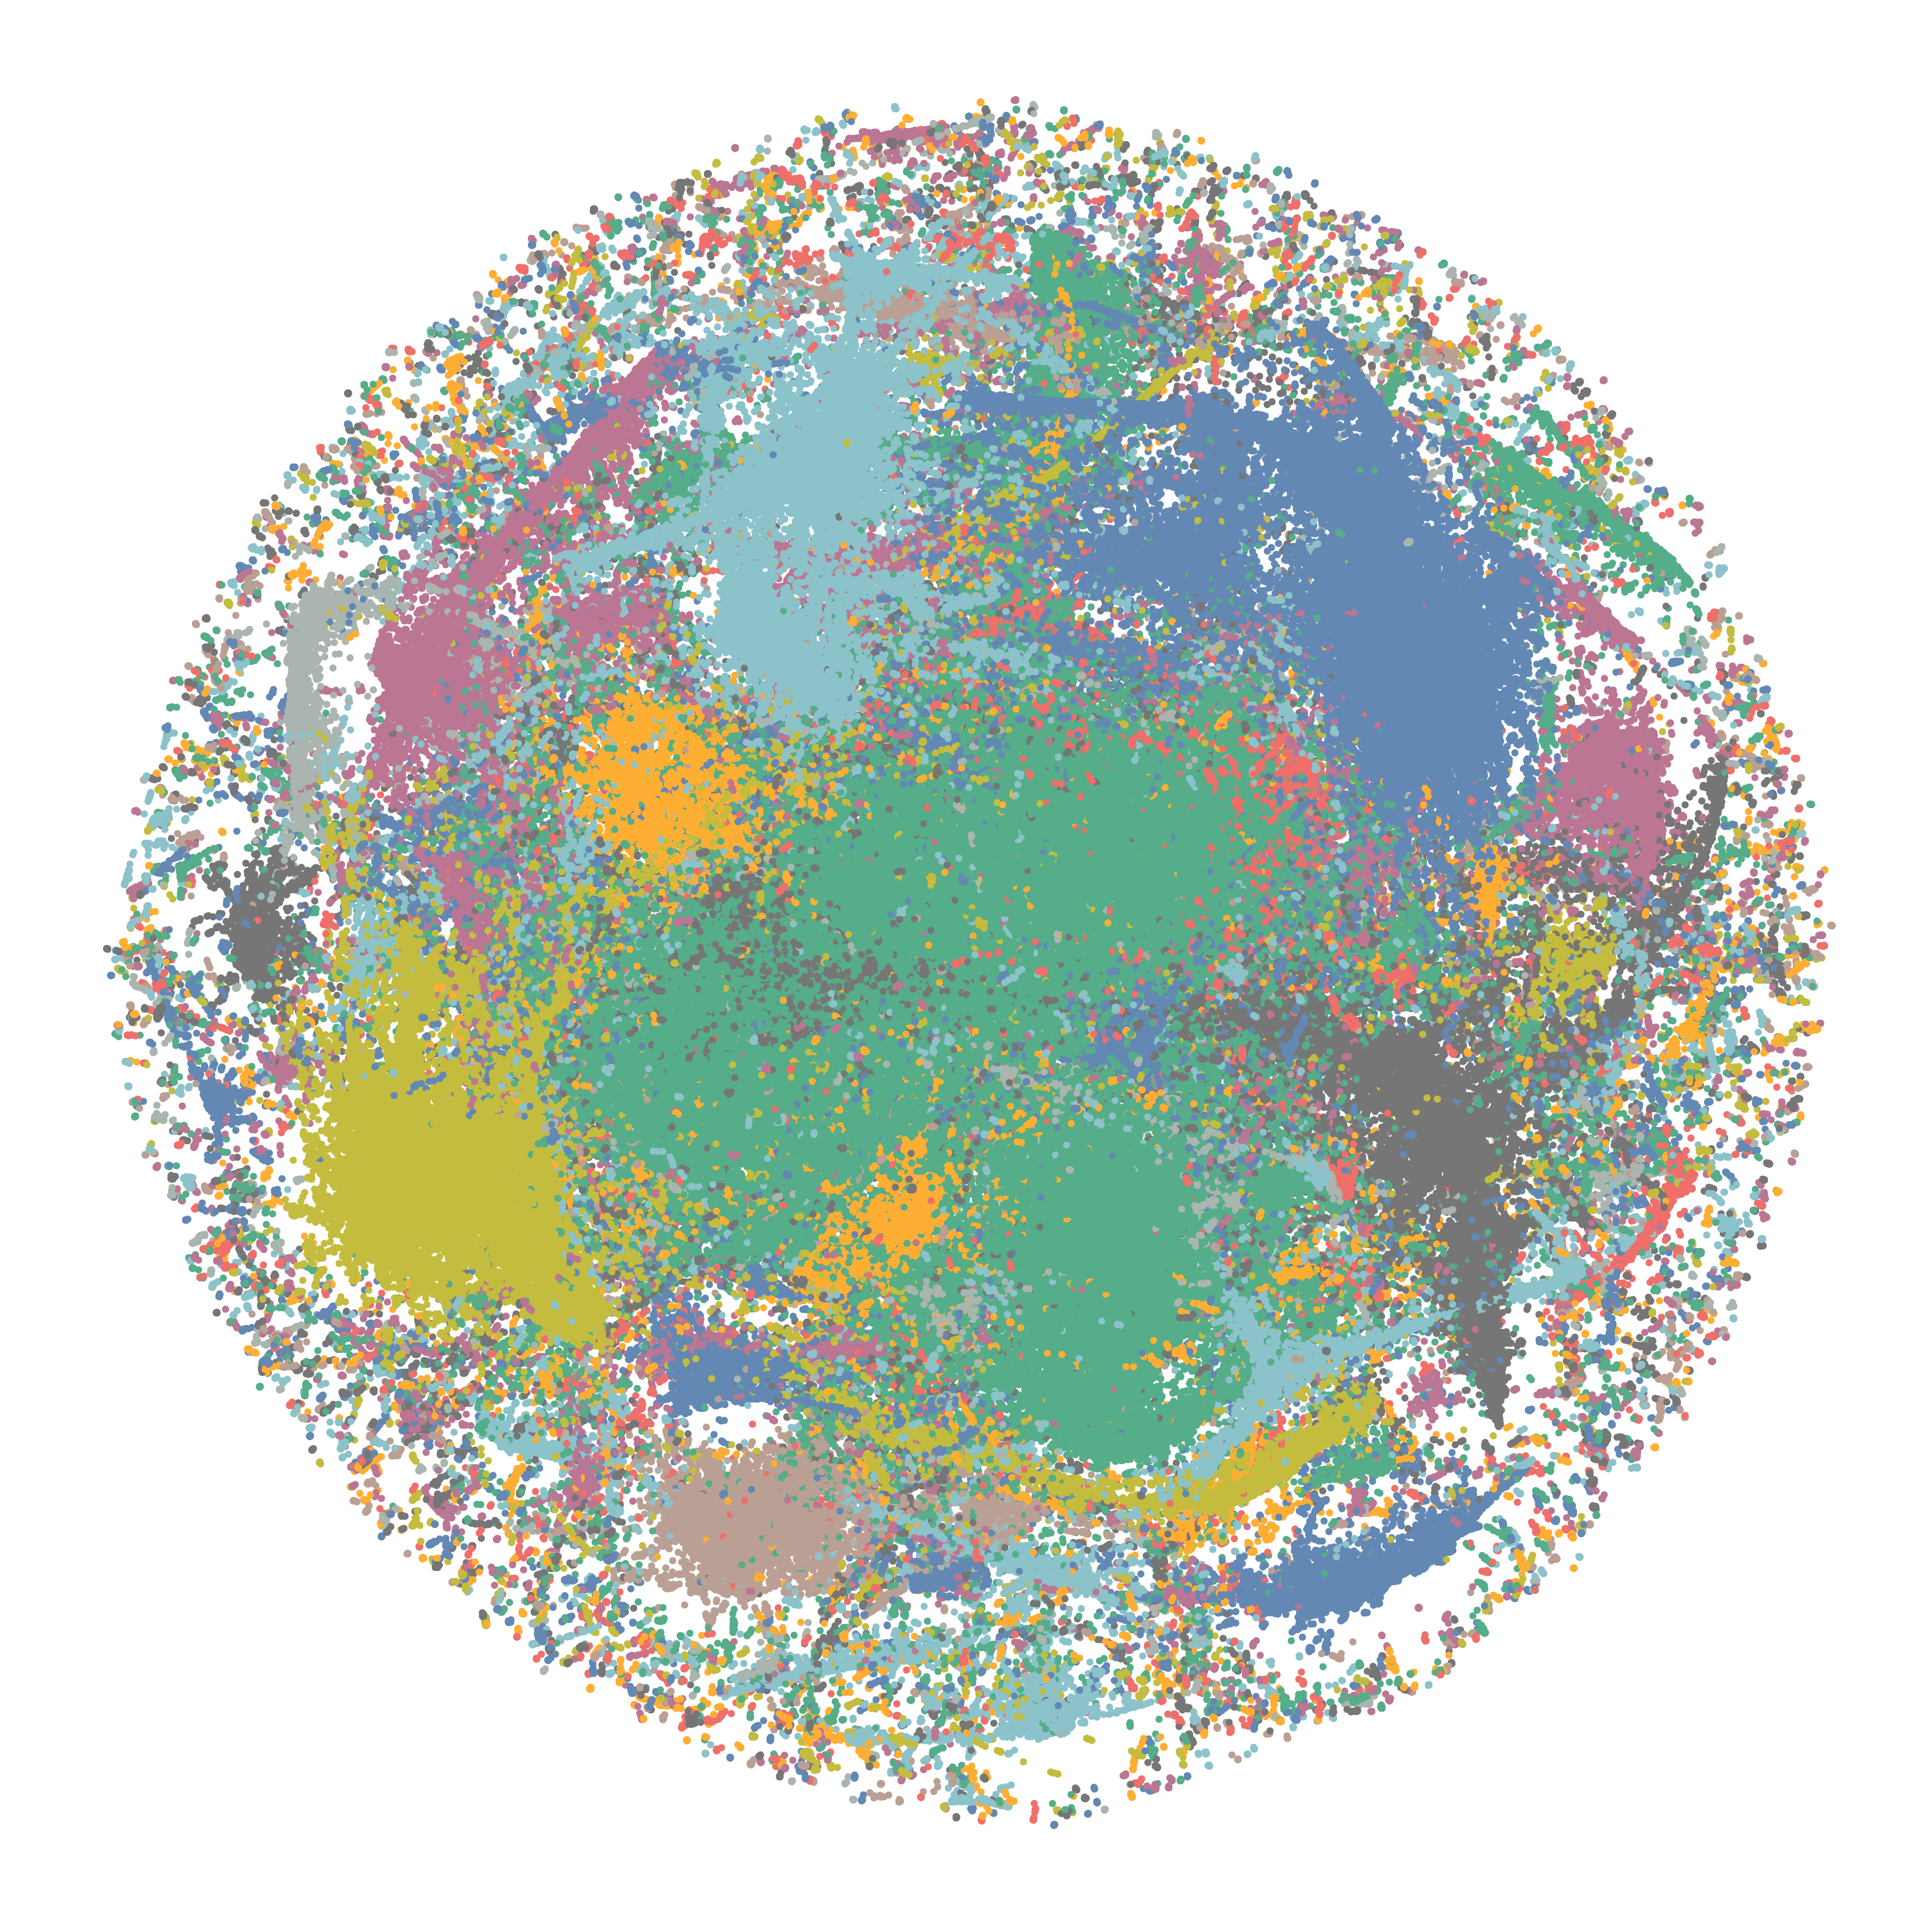
\includegraphics[width=\linewidth]{img/emb/bhtsne_hollywood}
    \caption{Barnes-Hut $t$-SNE}
  \end{subfigure}
\begin{subfigure}{0.45\linewidth}
  \centering
    \includegraphics[width=\linewidth]{img/emb/fitsne_hollywood}
    \caption{FI$t$-SNE}
\end{subfigure}
\par\bigskip
\begin{subfigure}{0.45\linewidth}
  \centering
    \includegraphics[width=\linewidth]{img/emb/ktsne_hollywood}
    \caption{$kt$-SNE}
\end{subfigure}
  \begin{subfigure}{0.45\linewidth}
    \centering
    \includegraphics[width=\linewidth]{img/emb/umap_hollywood}
    \caption{UMAP}
  \end{subfigure}
  \caption{hollywood}
\end{figure}

\begin{figure}[tbp]
  \centering
  \begin{subfigure}{0.45\linewidth}
    \centering
    \includegraphics[width=\linewidth]{img/emb/bhtsne_pubmed}
    \caption{Barnes-Hut $t$-SNE}
  \end{subfigure}
\begin{subfigure}{0.45\linewidth}
  \centering
    \includegraphics[width=\linewidth]{img/emb/fitsne_pubmed}
    \caption{FI$t$-SNE}
\end{subfigure}
\par\bigskip
\begin{subfigure}{0.45\linewidth}
  \centering
    \includegraphics[width=\linewidth]{img/emb/ktsne_pubmed}
    \caption{$kt$-SNE}
\end{subfigure}
  \begin{subfigure}{0.45\linewidth}
    \centering
    \includegraphics[width=\linewidth]{img/emb/umap_pubmed}
    \caption{UMAP}
  \end{subfigure}
  \caption{pubmed}
\end{figure}

\begin{figure}[tbp]
  \centering
  \begin{subfigure}{0.45\linewidth}
    \centering
    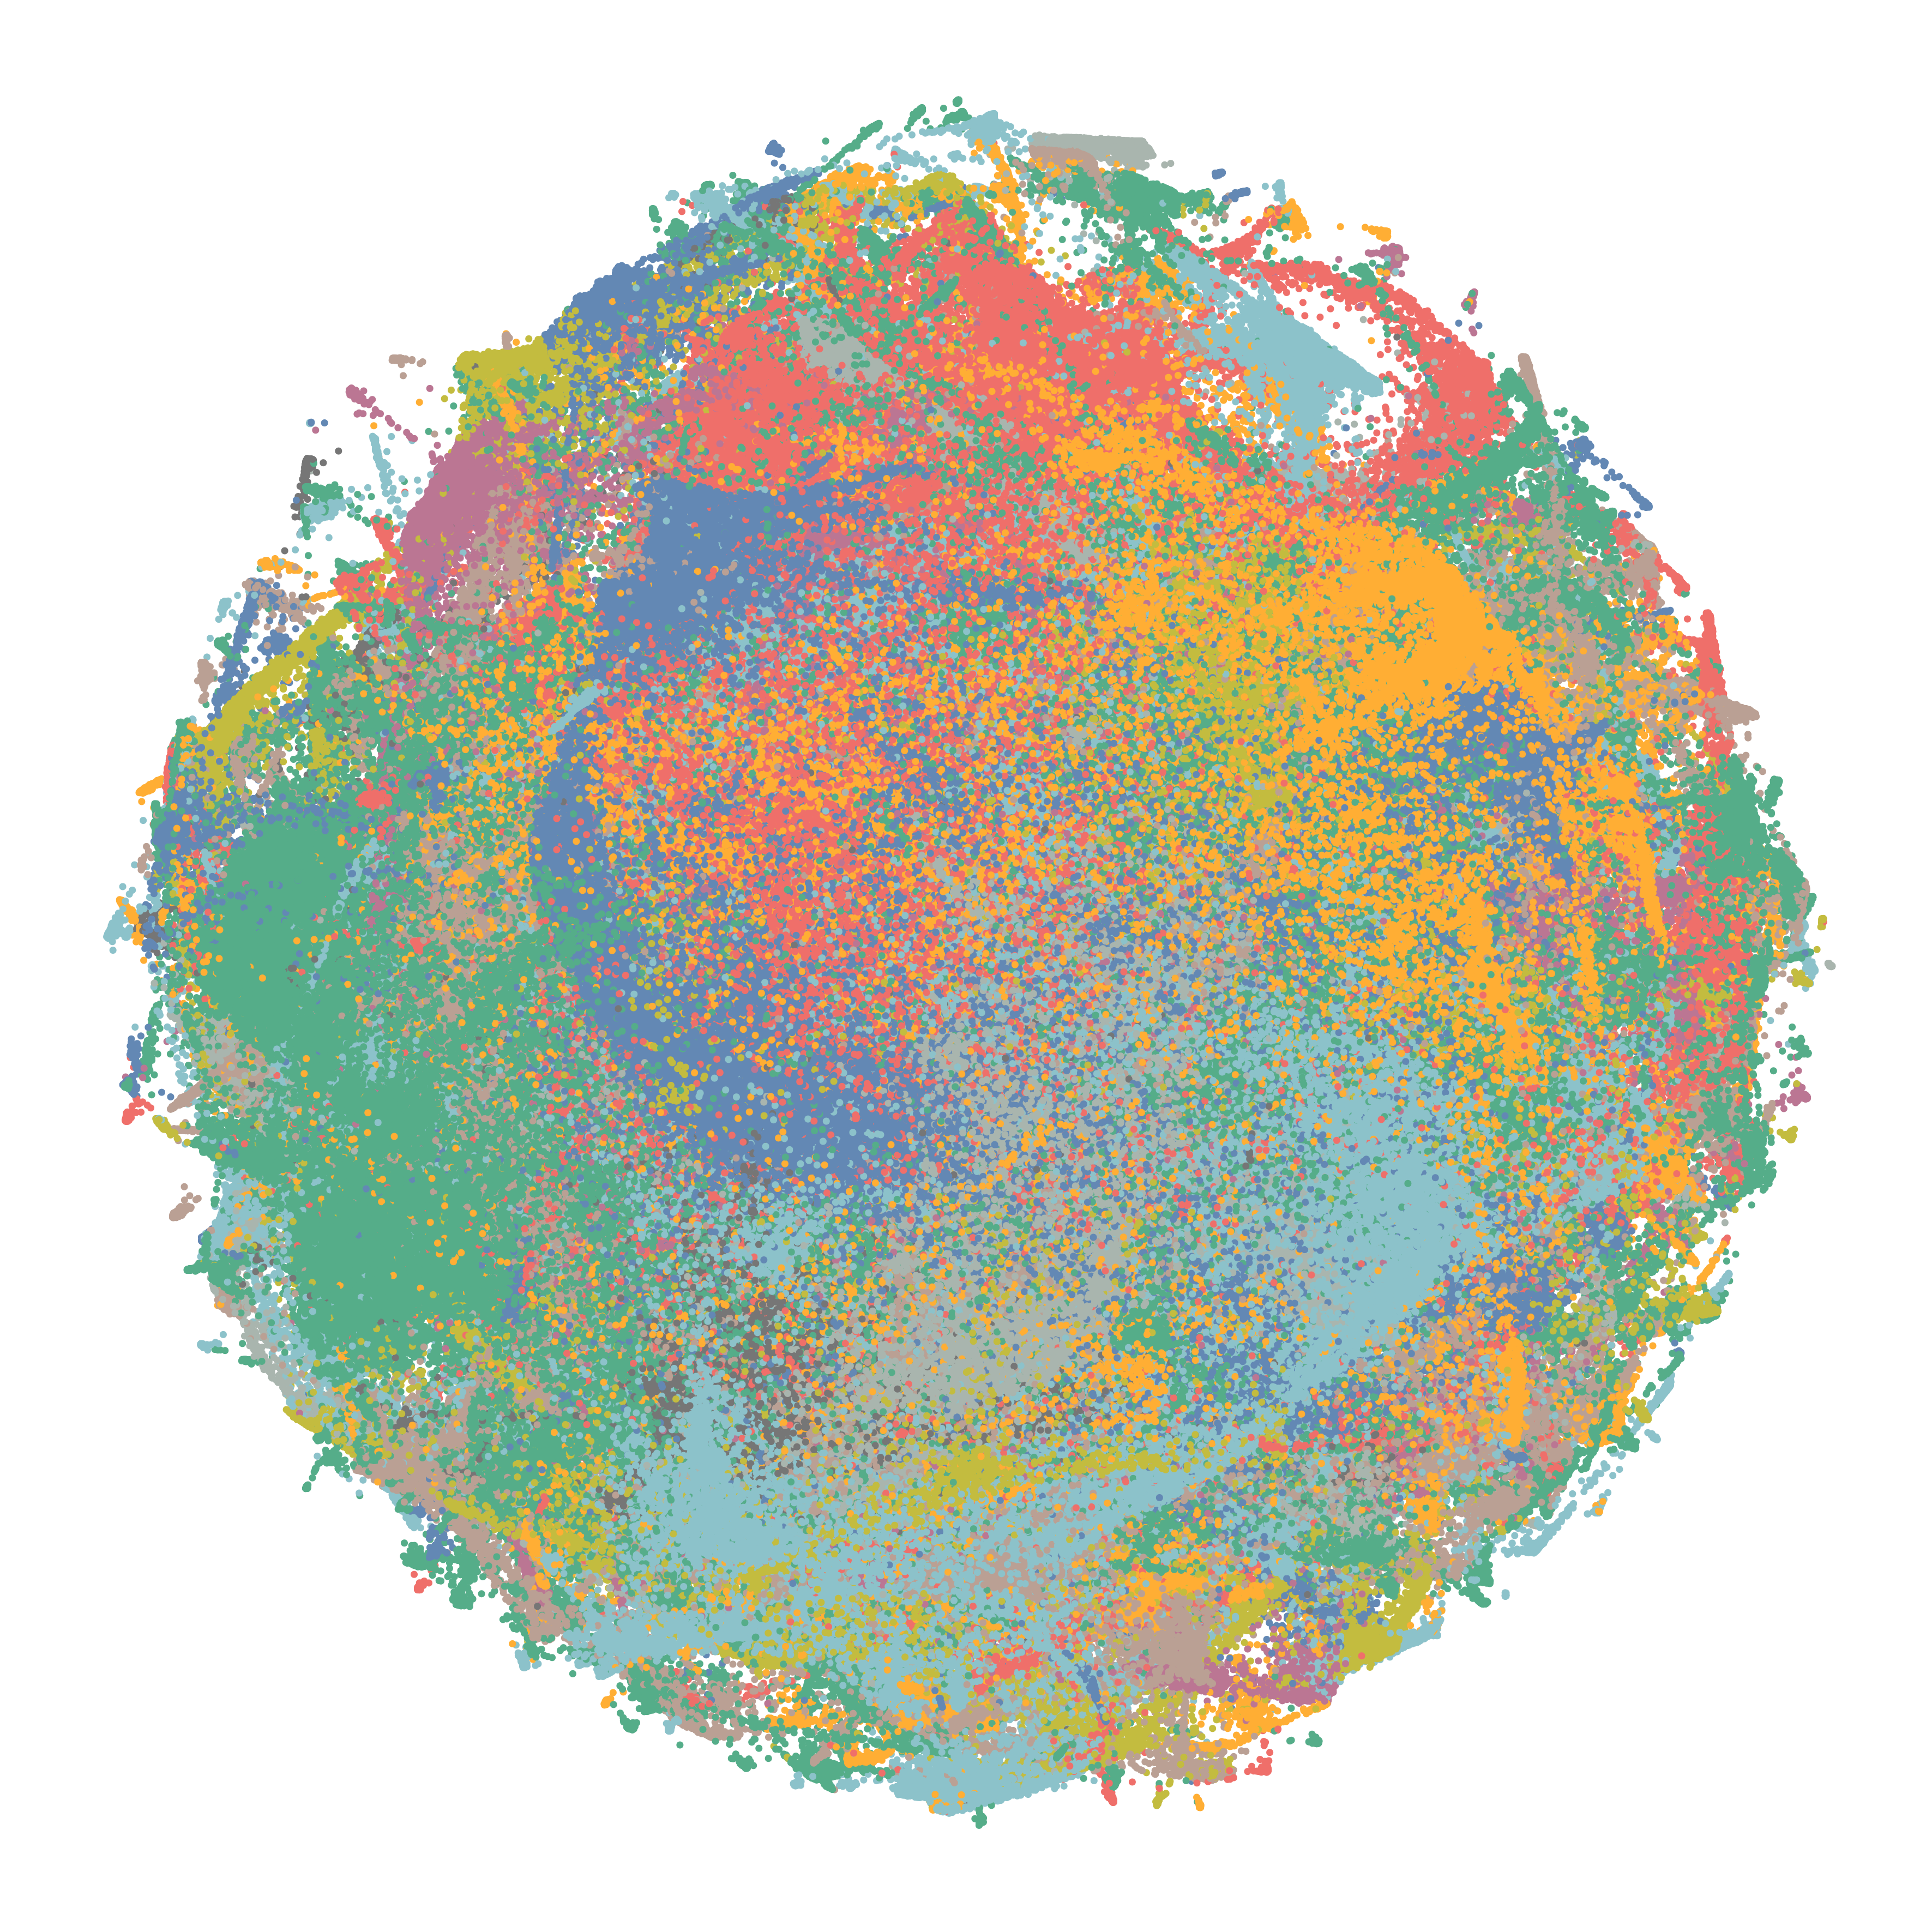
\includegraphics[width=\linewidth]{img/emb/bhtsne_wiki-topcats}
    \caption{Barnes-Hut $t$-SNE}
  \end{subfigure}
\begin{subfigure}{0.45\linewidth}
  \centering
    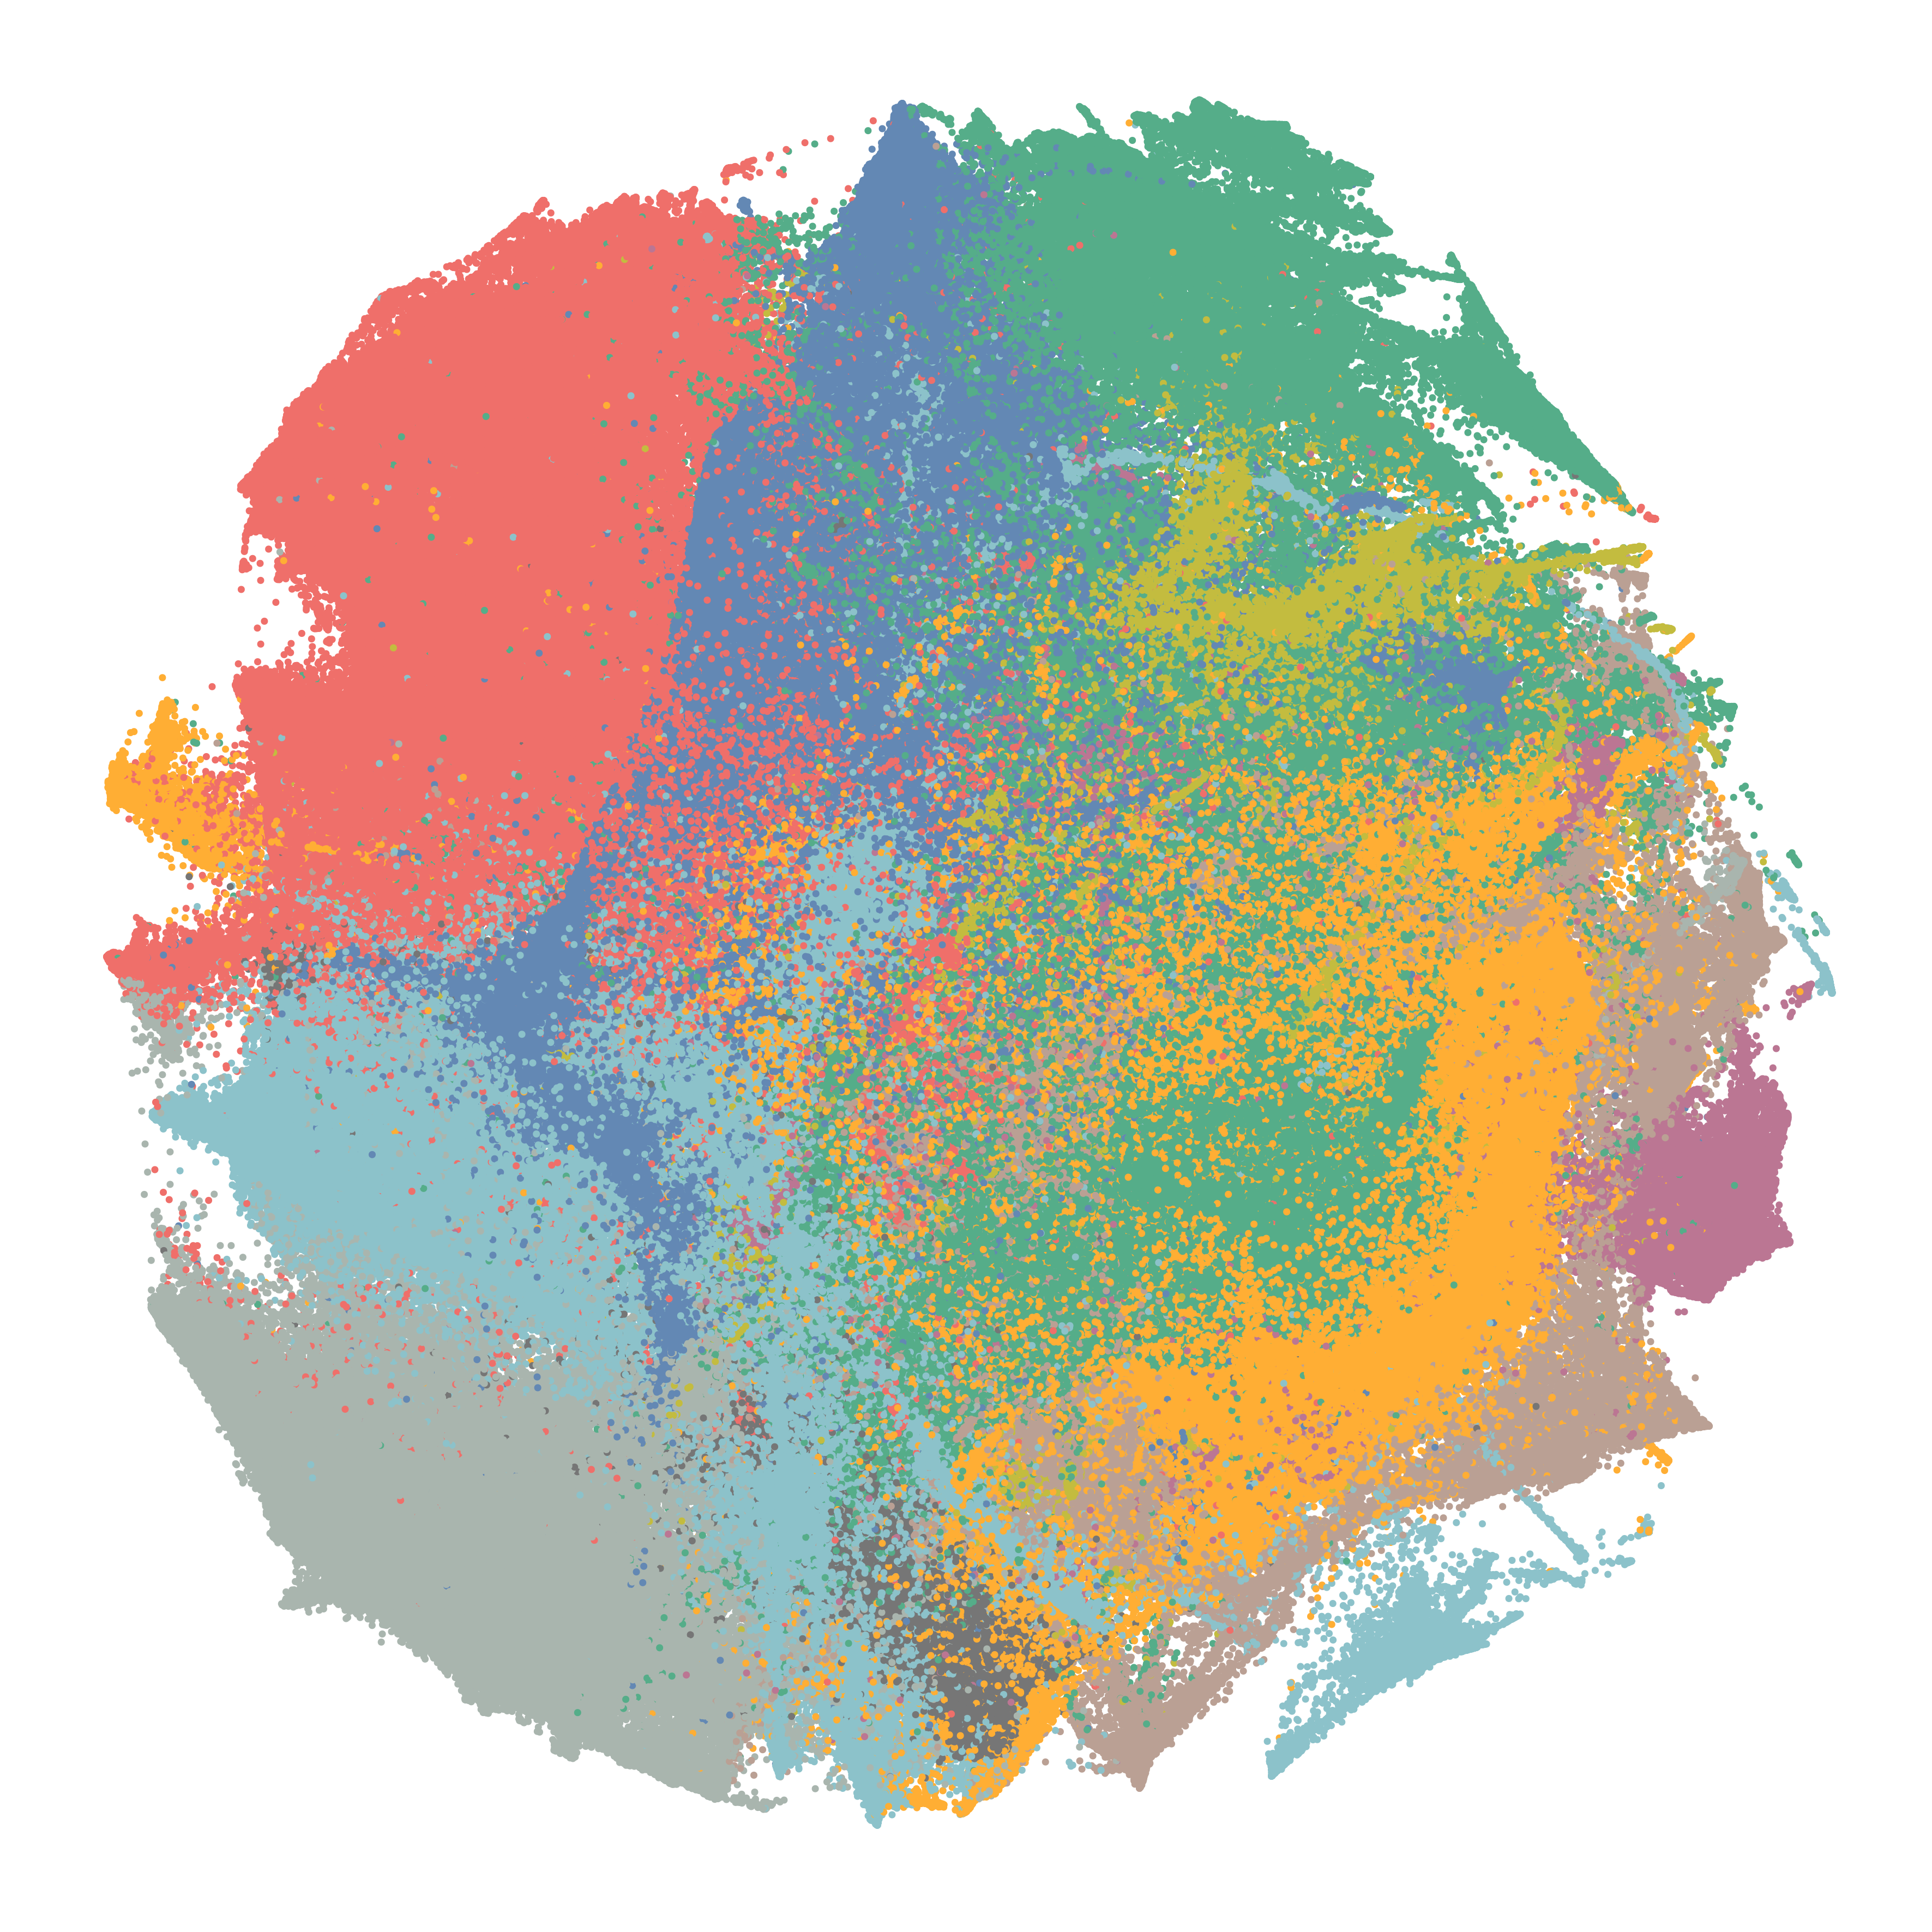
\includegraphics[width=\linewidth]{img/emb/fitsne_wiki-topcats}
    \caption{FI$t$-SNE}
\end{subfigure}
\par\bigskip
\begin{subfigure}{0.45\linewidth}
  \centering
    \includegraphics[width=\linewidth]{img/emb/ktsne_wiki-topcats}
    \caption{$kt$-SNE}
\end{subfigure}
  \begin{subfigure}{0.45\linewidth}
    \centering
    \includegraphics[width=\linewidth]{img/emb/umap_wiki-topcats}
    \caption{UMAP}
  \end{subfigure}
  \caption{wiki-topcats}
\end{figure}

\end{appendix}


% \backmatter
% \thispagestyle{empty} % no II on backside of title page

\end {document}
